% Transcribed from blueprint/src/parts/04-matern.tex.
\section{The \Matern{} pyramid}
\label{ch:matern}

Section~\ref{ch:pyramid} showed that covariance under one ratio admits many families, and that
between its knots a family is in general not fixed by its ladder. A designer who wants one pyramid
needs a further reason to choose. Scale-space theory gives such reasons as principles about what
smoothing may do to an image. On the line the classical principle is that smoothing creates no new
local extrema. The records of the line's \Matern{} pyramid obey it from rung to rung, for a suitable
class of inputs (Proposition~\ref{prop:ladder-non-creation-line}). In the plane this principle
fails. This section carries the \Matern{} pyramid to $\RR^d$, and gives a principle that holds in
the plane and selects it.

The pyramid is simple to describe. Its octave step from level $t$ to level $qt$ applies the
resolvent $(I - c^2t^2\Delta)^{-1}$, for a constant $c > 0$. The operator $I - c^2t^2\Delta$ is the
modified Helmholtz, or screened Poisson, operator. This section calls it the Helmholtz operator for
short, and its inverse the Helmholtz resolvent. Applying the resolvent to an image $u$ gives the
solution $v$ of $v - u = c^2t^2\Delta v$. That is one implicit Euler step, with the step size
$c^2t^2$, of the heat equation $\partial_\tau v = \Delta v$. So the pyramid runs the heat equation by
implicit steps, one per octave, and the step size grows by the factor $q^2$ from each octave to the
next.

The principle that selects it is a maximum principle for one such step. Required of every octave
step, it selects the \Matern{} pyramid among the isotropic families covariant under $q$, with the
scales labelled so that dilating the kernel at $t$ by $q$ gives the kernel at $qt$, up to a
relabelling in
$\mathcal{G}_q$. The subsections build to that result.
\begin{itemize}
\item Section~\ref{sec:matern-levels} constructs the pyramid in $\RR^d$ and looks at its octave
step as a computation.
\item Section~\ref{sec:matern-counting} shows that the line's reason for preferring the pyramid,
that it creates no extrema, does not carry to $d \ge 2$.
\item Section~\ref{sec:matern-selection} gives a reason that does. \emph{Non-enhancement} of local
extrema requires that smoothing not raise a local maximum or lower a local minimum. Read at one
finite step, it holds among the symmetric rotation-invariant laws exactly for the Helmholtz
resolvents $(I - \tau\Delta)^{-1}$, $\tau \ge 0$, the identity among them
(Proposition~\ref{prop:stage-lemma}). Then take an isotropic family covariant under $q$, in the
canonical discrete gauge. Required of one octave step, the principle fixes only the ladder through
it. Required of every octave step $\mu_{t,qt}$, from every scale $t \in [1, q)$, it selects the
\Matern{} pyramid up to the gauge $\chi \in \mathcal{G}_q$
(Theorem~\ref{thm:selection-stratum-two}(1)--(2)).
\end{itemize}

The section compares the plane with the line throughout. The statements on the line that it cites
are proved in Section~\ref{ch:line-appendix} of the supplement.
\begin{itemize}
\item The \Matern{} pyramid on the line, with its octave identity, generator and limit
$q \downarrow 1$ (Theorem~\ref{thm:matern-pyramid-line}).
\item Its \Polya{} frequency kernels and steps (Theorem~\ref{thm:matern-pyramid-line-noncreation}).
\item The counts from rung to rung (Proposition~\ref{prop:ladder-non-creation-line}).
\item The sums of Laplace atoms, the exponents $\log(1 + \omega^2/\vartheta^2)$ of two-sided
exponential laws, which are admissible when $\sum_i\vartheta_i^{-2} < \infty$
(Lemma~\ref{lem:laplace-atoms-admissible}).
\item The selection by phase entropy (Theorem~\ref{thm:phase-entropy-selection}).
\end{itemize}

\subsection{The levels and the octave step}
\label{sec:matern-levels}

What are the levels of the \Matern{} pyramid in $\RR^d$, and what must a pyramid compute to
produce them? The answer starts from the octave step, builds the family from it, and then looks at
the octave step again as a computation.
\begin{itemize}
\item The octave step: the law $L_r$, its density, and the profile $b_d$ of its \Levy{} measure
(Definition~\ref{def:matern-pyramid-data}, Lemmas~\ref{lem:bessel-profile}
and~\ref{lem:bessel-k}).
\item The pyramid: its existence and uniqueness, its projections onto lines, its generator and its
limit as $q \downarrow 1$ (Theorem~\ref{thm:matern-pyramid}).
\item The steps between scales that are not a factor $q$ apart, and what becomes of the line's
Thorin property in the plane (Propositions~\ref{prop:matern-increments}
and~\ref{prop:thorin-in-dimension-d}).
\item The octave step as a computation. In $d \ge 2$ it does not split into first-order passes and
its density has no central value. In every dimension the difference of two levels is a Laplacian
(Lemma~\ref{lem:no-first-order-factorization}, Propositions~\ref{prop:matern-generator-octave}
and~\ref{prop:laplacian-pyramid}).
\item A separable twin, the frame \Matern{} pyramid, which the next two subsections compare with the
\Matern{} pyramid (Definition~\ref{def:frame-matern-pyramid}).
\end{itemize}

The octave step is the law $L_r$ with transform $(1 + r^2|\omega|^2)^{-1}$, at $r = ct$. The
literature knows it under several names, and they all denote this one law. Its density is
$r^{-d}G_2(x/r)$, with $G_2$ the Bessel potential of order $2$, the kernel of $(I - \Delta)^{-1}$
[\sscite{stein1970singular}, Ch.~V, \S 3, (26) and Prop.~2, p.~132], read in this paper's
convention for the transform. So $L_r$ is the Green's function of $I - r^2\Delta$. It is also the
\Matern{} law of index $1$ at range $r$. The laws with transform $(1 + r^2|\omega|^2)^{-\gamma}$ are
named after the \Matern{} covariances of spatial statistics
[\sscite{whittle1954stationary}, p.~448; \sscite{lindgren2011explicit}, (2), p.~426], and for $\gamma > d/2$ their
densities are those covariances (Section~\ref{ch:price}). In $d \ge 2$ the density of the octave
step, of index $1 \le d/2$, is not a \Matern{} covariance. No kernel $\mu_t$ of the \Matern{}
pyramid is a \Matern{} law, in any dimension. Read as a function of $|\omega|^2$, its transform is
singular at infinitely many points of the negative axis, and a \Matern{} transform at one. Finally, $L_r$ is the kernel of
\prog{iso v0.1}{Prop.~3.12(2), p.~16} at scale $\sqrt2\,r$. The paper writes $L_r$ for the law,
and the Helmholtz resolvent for the operator $f \mapsto L_r * f$. The name Bessel potential stays in
use for $L_r$ where the comparison with the literature needs it.

The definition below starts from one more description. The law $L_r$ is a Gaussian variance
mixture: the position at an exponential random time of a Brownian motion whose law at time $s$ is
$N(0, 2sI)$, the heat kernel of $\partial_\tau v = \Delta v$ at time $s$. This is the simplest case of
\emph{subordination}, which runs Brownian motion at a random time. The mixture gives the transform
and the density of $L_r$ at once. The definition also introduces the two functions that the rest of
the subsection uses. The exponent $F_q$ of the \Matern{} pyramid is the sum of the exponents of its
octave steps at the finer scales. The function $b_d$ describes the \Levy{} measure of $L_1$ in polar
coordinates. It is the polar profile of $L_1$, in the sense of Section~\ref{ch:cited}, and
$b_d(\cdot/r)$ is that of $L_r$ (Lemma~\ref{lem:bessel-profile}(2)).

% shared with blueprint def:matern-pyramid-data
\begin{definition}[the octave step and the \Matern{} exponent]
\label{def:matern-pyramid-data}

Fix $d \ge 1$. For $r > 0$ let
\[
  L_r := \int_0^\infty e^{-s}\,N(0, 2sr^2I)\,ds ,
\]
the law of $r\sqrt{2X}\,Z$ with $X$ standard exponential and $Z$ standard normal on $\RR^d$
independent of it. Call $L_r$ the \emph{\Matern{} law of index $1$ at range $r$}, and write $L_r$
also for the operator $f \mapsto L_r * f$. For $q > 1$ and $c > 0$ put
\[
  F_q(r) := \sum_{i \ge 1}\log\bigl(1 + c^2q^{-2i}r^2\bigr), \qquad
  b_d(y) := \frac{2}{\Gamma(d/2)}\int_0^\infty v^{d/2-1}e^{-v-y^2/(4v)}\,dv ,
  \qquad r, y \ge 0 .
\]
The series converges, each term being at most $c^2q^{-2i}r^2$.
\end{definition}

% shared with blueprint lem:bessel-profile
\begin{lemma}[the octave step and its profile]
\label{lem:bessel-profile}

Let $d \ge 1$ and $r > 0$.
\begin{enumerate}
\item $\widehat{L_r}(\omega) = (1 + r^2|\omega|^2)^{-1}$. The law $L_r$ has the density
$r^{-d}G(x/r)$, where
\[
  G(x) := \int_0^\infty e^{-s}(4\pi s)^{-d/2}e^{-|x|^2/(4s)}\,ds \in (0, \infty]
\]
is continuous on $\RR^d \setminus \{0\}$. For every $g \in L^1(\RR^d)$,
$(I - r^2\Delta)(L_r * g) = g$ in the sense of distributions.
\item For every $\beta > 0$ and $\omega \in \RR^d$,
\[
  \log\bigl(1 + \beta|\omega|^2\bigr)
   = \int_{\RR^d}\bigl(1 - \cos\langle\omega, x\rangle\bigr)\,
     \frac{b_d(|x|/\sqrt\beta)}{|S^{d-1}|\,|x|^d}\,dx .
\]
\item $b_d(0) = 2$, and $b_d$ is continuous and strictly decreasing on $[0, \infty)$, with
$b_d(y) \le C_de^{-y/2}$, $C_d := 2^{1+d/2}$. Further $b_1(y) = 2e^{-y}$ and
$b_3(y) = 2(1 + y)e^{-y}$.
\end{enumerate}
\end{lemma}

\begin{proof}
\emph{(1)} The law $L_r$ is the image of $L_1$ under $x \mapsto rx$, and $L_1$ is the law of
$\sqrt{2X}\,Z$. Given $X = s$, the vector $\sqrt{2s}\,Z$ has the law $N(0, 2sI)$, with the transform
$e^{-s|\omega|^2}$ and the density $g_{2s}(x) := (4\pi s)^{-d/2}e^{-|x|^2/(4s)}$. Integrating against
$e^{-s}\,ds$ gives, by Tonelli's theorem, the transform
$\int_0^\infty e^{-s(1 + |\omega|^2)}\,ds = (1 + |\omega|^2)^{-1}$ of $L_1$. The function
$G = \int_0^\infty e^{-s}g_{2s}\,ds$ is integrable, and by Fubini's theorem its transform is the same
integral, $(1 + |\omega|^2)^{-1}$. By the uniqueness of the transform, $L_1$ has the density $G$.
The image under $x \mapsto rx$ then has the density $r^{-d}G(x/r)$ and the transform
$(1 + r^2|\omega|^2)^{-1}$. For $|x| \ge \delta > 0$ the integrand defining $G$ is at most
$e^{-s}(4\pi s)^{-d/2}e^{-\delta^2/(4s)}$, which is integrable in $s$. So $G$ is finite off the
origin, and, differentiating under the integral sign in $|x|^2$, it is smooth there.

For the Green's function let $g \in L^1(\RR^d)$, let $\varphi$ be real, smooth and of compact
support, and put $\psi := \varphi - r^2\Delta\varphi$. First, for every $z$,
\[
  \int\psi(z + y)\,L_r(dy) = \varphi(z) .
\]
Read $\varphi$ as a complex Schwartz function, and write $\mathcal{F}$ for the transform of the
$2\pi$ convention, $\mathcal{F}\varphi(\xi) := \int e^{-2\pi i\langle\xi, x\rangle}\varphi(x)\,dx =
\widehat\varphi(-2\pi\xi)$. Fourier inversion gives
$\varphi(x) = \int e^{2\pi i\langle\xi, x\rangle}\mathcal{F}\varphi(\xi)\,d\xi$, and the transform of
$\Delta\varphi$ is $-4\pi^2|\xi|^2\mathcal{F}\varphi$, so
$\psi(x) = \int e^{2\pi i\langle\xi, x\rangle}(1 + 4\pi^2r^2|\xi|^2)\mathcal{F}\varphi(\xi)\,d\xi$, an
absolutely convergent integral. By Fubini's theorem,
\[
  \int\psi(z + y)\,L_r(dy)
   = \int e^{2\pi i\langle\xi, z\rangle}(1 + 4\pi^2r^2|\xi|^2)\mathcal{F}\varphi(\xi)\,
     \widehat{L_r}(2\pi\xi)\,d\xi
   = \int e^{2\pi i\langle\xi, z\rangle}\mathcal{F}\varphi(\xi)\,d\xi = \varphi(z) .
\]
Second, $\psi$ is bounded, so $(x, y) \mapsto g(x - y)\psi(x)$ is integrable for
the product of $dx$ and $L_r(dy)$. Fubini's theorem and the translation $x = z + y$ give
\[
  \int(L_r * g)\,\psi = \int\int g(x - y)\psi(x)\,dx\,L_r(dy)
   = \int\int g(z)\psi(z + y)\,dz\,L_r(dy) = \int g(z)\varphi(z)\,dz .
\]
This is $(I - r^2\Delta)(L_r * g) = g$ in the sense of distributions.

\emph{(2)} Frullani's integral gives, for $u \ge 0$,
\[
  \log(1 + \beta u) = \int_0^\infty\bigl(1 - e^{-su}\bigr)\,e^{-s/\beta}\,\frac{ds}{s} .
\]
Both sides vanish at $u = 0$. For $u > 0$ put $a := 1/\beta$ and $b := u + 1/\beta$. The integrand is
$(e^{-as} - e^{-bs})/s = \int_a^be^{-ts}\,dt$, and Tonelli's theorem gives
$\int_a^b\int_0^\infty e^{-ts}\,ds\,dt = \int_a^bdt/t = \log(b/a) = \log(1 + \beta u)$.
Put $u = |\omega|^2$. Let $g_{2s}(x) := (4\pi s)^{-d/2}e^{-|x|^2/(4s)}$ be the density of
$N(0, 2sI)$. It is symmetric with mass $1$, so
$1 - e^{-s|\omega|^2} = \int(1 - \cos\langle\omega, x\rangle)\,g_{2s}(x)\,dx$. All integrands are
nonnegative, and Tonelli's theorem gives
$\log(1 + \beta|\omega|^2) = \int(1 - \cos\langle\omega, x\rangle)\,f_\beta(|x|)\,dx$ with
\[
  f_\beta(\rho) := \int_0^\infty(4\pi s)^{-d/2}e^{-\rho^2/(4s)}e^{-s/\beta}\,\frac{ds}{s} ,
  \qquad \rho > 0 .
\]
The substitution $s = \rho^2/(4v)$ has $ds/s = -dv/v$ and $(4\pi s)^{-d/2} = \pi^{-d/2}\rho^{-d}v^{d/2}$,
so $f_\beta(\rho) = \pi^{-d/2}\rho^{-d}\int_0^\infty v^{d/2-1}e^{-v-\rho^2/(4\beta v)}\,dv$. With
$|S^{d-1}| = 2\pi^{d/2}/\Gamma(d/2)$ this reads $|S^{d-1}|\,\rho^df_\beta(\rho) = b_d(\rho/\sqrt\beta)$.

\emph{(3)} At $y = 0$ the integral is $\Gamma(d/2)$, so $b_d(0) = 2$. For each $v > 0$ the integrand
is continuous and strictly decreasing in $y \ge 0$ and at most $v^{d/2-1}e^{-v}$, so $b_d$ is
continuous by dominated convergence and strictly decreasing. For the bound, split the exponent in
halves. The inequality of the means gives $\tfrac12\bigl(v + y^2/(4v)\bigr) \ge y/2$, and dropping
a term gives $\tfrac12\bigl(v + y^2/(4v)\bigr) \ge v/2$. So the integrand is at most
$e^{-y/2}v^{d/2-1}e^{-v/2}$, and
$b_d(y) \le e^{-y/2}\,\frac{2}{\Gamma(d/2)}\int_0^\infty v^{d/2-1}e^{-v/2}\,dv = 2^{1+d/2}e^{-y/2}$.

For the closed forms let $y > 0$; at $y = 0$ both read $b_d(0) = 2$. Put $\eta := y/2$ and
$E(w) := e^{-w^2 - \eta^2/w^2}$ for $w > 0$. The substitution $v = w^2$ gives
\[
  \int_0^\infty v^{\nu-1}e^{-v-y^2/(4v)}\,dv = 2\int_0^\infty w^{2\nu-1}E(w)\,dw .
\]
Since $w^2 + \eta^2/w^2 = 2\eta + (w - \eta/w)^2$, $E(w) = e^{-2\eta}e^{-(w - \eta/w)^2}$. Put
\[
  J_1 := \int_0^\infty e^{-(w - \eta/w)^2}\,dw , \qquad
  J_2 := \int_0^\infty \eta w^{-2}e^{-(w - \eta/w)^2}\,dw .
\]
The substitution $w \mapsto \eta/w$ maps $(0, \infty)$ onto itself and leaves $(w - \eta/w)^2$
unchanged, so $J_1 = J_2$. The map $\sigma(w) := w - \eta/w$ is an increasing bijection of
$(0, \infty)$ onto $\RR$ with the derivative $1 + \eta w^{-2}$, so
$J_1 + J_2 = \int_{\RR}e^{-\sigma^2}\,d\sigma = \sqrt\pi$. Hence $J_1 = J_2 = \tfrac12\sqrt\pi$, and
\[
  \int_0^\infty E(w)\,dw = \tfrac12\sqrt\pi\,e^{-2\eta} , \qquad
  \int_0^\infty w^{-2}E(w)\,dw = \frac{\sqrt\pi}{2\eta}\,e^{-2\eta} .
\]
At $\nu = 1/2$, with $\Gamma(1/2) = \sqrt\pi$, this gives
$b_1(y) = \frac{2}{\sqrt\pi}\cdot2\int_0^\infty E = 2e^{-y}$. At $\nu = 3/2$ the integral
$\int_0^\infty w^2E(w)\,dw$ is needed. The function $F(w) := wE(w)$ has the derivative
$F'(w) = (1 - 2w^2 + 2\eta^2w^{-2})E(w)$, and $F(w) \to 0$ as $w \to 0$ from above and as
$w \to \infty$, since $0 \le E(w) \le e^{-w^2}$. So $\int_0^\infty F' = 0$, that is
\[
  2\int_0^\infty w^2E(w)\,dw = \int_0^\infty E(w)\,dw + 2\eta^2\int_0^\infty w^{-2}E(w)\,dw
   = \tfrac12\sqrt\pi\,e^{-2\eta}(1 + 2\eta) .
\]
With $\Gamma(3/2) = \sqrt\pi/2$ this gives
$b_3(y) = \frac{4}{\sqrt\pi}\cdot\tfrac12\sqrt\pi\,(1 + y)e^{-y} = 2(1 + y)e^{-y}$.
\end{proof}

In the plane the profile is a modified Bessel function [\sscite{dlmf2026}], $b_2(y) = 2yK_1(y)$. The
next lemma gives this form in every dimension. It also proves the facts on $K_0$ that two later
proofs use: the limit profile in the plane, and the value of the density at its centre
(Propositions~\ref{prop:thorin-in-dimension-d} and~\ref{prop:matern-generator-octave}).

% shared with blueprint lem:bessel-k
\begin{lemma}[the profile through Bessel functions]
\label{lem:bessel-k}

Let $K_\nu$ be the modified Bessel function of the second kind of order $\nu$, and let $y > 0$.
\begin{enumerate}
\item For every real $\nu$,
\[
  \int_0^\infty v^{\nu-1}e^{-v-y^2/(4v)}\,dv = 2(y/2)^\nu K_\nu(y) .
\]
So $b_d(y) = \frac{4}{\Gamma(d/2)}(y/2)^{d/2}K_{d/2}(y)$, and $b_2(y) = 2yK_1(y)$.
\item $K_0$ is differentiable on $(0, \infty)$ with $K_0' = -K_1$, and $K_0(y) \to 0$ as
$y \to \infty$.
\item $K_0(y) = \int_1^\infty e^{-ys}(s^2 - 1)^{-1/2}\,ds$, and $K_0(y) - \log(1/y)$ stays bounded
as $y \downarrow 0$.
\end{enumerate}
\end{lemma}

\begin{proof}
\emph{(1)} DLMF~10.32.10 (\ledger{A51}), at $z = y$ and at the order $-\nu$, gives
$K_{-\nu}(y) = \tfrac12(\tfrac12y)^{-\nu}\int_0^\infty t^{\nu-1}e^{-t - y^2/(4t)}\,dt$. By
DLMF~10.32.9, $K_\nu(y) = \int_0^\infty e^{-y\cosh u}\cosh(\nu u)\,du$, which is even in $\nu$, so
$K_{-\nu} = K_\nu$ and the identity follows. The integral converges for every real $\nu$. The
substitution $v = \tfrac y2e^w$, under which $v + y^2/(4v) = y\cosh w$ and $dv/v = dw$, turns it into
$2(\tfrac y2)^\nu\int_0^\infty\cosh(\nu w)e^{-y\cosh w}\,dw$, and
$\cosh(\nu w)e^{-y\cosh w} \le e^{2\nu^2/y}e^{-(y/8)w^2}$ for $w \ge 0$, since
$\cosh(\nu w) \le e^{|\nu|w}$ and $\cosh w \ge w^2/4$. At $\nu = d/2$ the identity is the closed form
of $b_d$. At $d = 2$, $\Gamma(1) = 1$ gives $b_2(y) = 2yK_1(y)$.

\emph{(2)} By DLMF~10.32.9, $K_0(z) = \int_0^\infty e^{-z\cosh u}\,du$. For $|z - y| < y/2$ the
$z$-derivative of the integrand, $-\cosh u\,e^{-z\cosh u}$, is at most
$\cosh u\,e^{-(y/2)\cosh u}$ in absolute value, and the integral of this bound is $K_1(y/2)$, which is
finite by the bound in (1). So $K_0$ is differentiable at $y$ with
$K_0'(y) = -\int_0^\infty\cosh u\,e^{-y\cosh u}\,du = -K_1(y)$. For $y \ge 1$,
$(y - 1)(\cosh u - 1) \ge 0$ gives $y\cosh u \ge (y - 1) + \cosh u$, so
$0 \le K_0(y) \le e^{1-y}K_0(1)$, which tends to $0$ as $y \to \infty$.

\emph{(3)} The substitution $s = \cosh u$, with $ds = \sinh u\,du$ and
$\sinh u = (s^2 - 1)^{1/2}$, maps $(0,\infty)$ onto $(1,\infty)$ and turns
$K_0(y) = \int_0^\infty e^{-y\cosh u}\,du$ into the integral of (3), which therefore converges. For the
origin let $0 < y < 1$ and $L := \log(1/y) > 0$, so that $ye^L = 1$. On $(0, L]$ the integrand lies
between $1 - y\cosh u \ge 1 - ye^u$ and $1$, since $\cosh u \le e^u$. On $(L, \infty)$ it is positive
and, since $y\cosh u \ge \tfrac12ye^u = \tfrac12e^{u-L} \ge \tfrac12(u - L)$, at most
$e^{-(u-L)/2}$, whose integral over $(L,\infty)$ is $2$. Hence
\[
  L - (1 - y) = \int_0^L\bigl(1 - ye^u\bigr)\,du \le K_0(y) \le L + 2 ,
\]
and $|K_0(y) - \log(1/y)| \le 2$ for $0 < y < 1$.

The one cited fact is DLMF~10.32.10 (\ledger{A51}), read in (1); DLMF~10.32.9 is the definition of
$K_\nu$.
\end{proof}

The pyramid is built from these pieces. Its exponent at scale $t$ is $F_q(t|\omega|)$, the sum of
the exponents of the octave steps below $t$. The series telescopes,
$F_q(qr) - F_q(r) = \log(1 + c^2r^2)$, so the step from $t$ to $qt$ is the one law $L_{ct}$. The
next theorem shows that this exponent defines an isotropic family, covariant under every dilation.
Among continuous $F$ with $F(0) = 0$, the octave identity determines the exponent. Clause (1)
places $F_q$ in the class $\mathcal{A}_d$ of Section~\ref{subsec:cited-d}, the admissible $F$ for
which $F(|\cdot|)$ is the exponent of a self-decomposable law on $\RR^d$. The proof checks this
through the polar form of $\mathcal{A}_d$ (Theorem~\ref{thm:cited-A35}). The other clauses record
what later results use. They are the projections onto lines, where the line's counts survive for
suitable inputs, the generator, and the limit $q \downarrow 1$.

% shared with blueprint thm:matern-pyramid
\begin{theorem}[the \Matern{} pyramid in $\RR^d$]
\label{thm:matern-pyramid}

Fix $q > 1$, $c > 0$ and $d \ge 1$.
\begin{enumerate}
\item \emph{(Admissibility.)} $F_q \in \mathcal{A}_d$, with Gaussian coefficient $0$ and the
nonincreasing polar profile $k_d(r) = \sum_{i \ge 1}b_d(rq^i/c)$. So the transforms
$\exp\bigl[-\bigl(F_q(t|\omega|) - F_q(s|\omega|)\bigr)\bigr]$, $0 \le s \le t$, define an isotropic
family with $S_\lambda t = \lambda t$ for every $\lambda > 0$, the \emph{\Matern{} pyramid}. Its
octave step is one Bessel potential, $\mu_{t,qt} = L_{ct}$ for $t > 0$. Its kernel is the Gaussian variance
mixture $\mu_t = \mathrm{law}\bigl(\sqrt{2V_t}\,Z\bigr)$, with
$V_t = \sum_{i \ge 1}c^2q^{-2i}t^2X_i$, the $X_i$ independent standard exponential and $Z$ standard
normal on $\RR^d$ independent of them, and for $t > 0$ it has a $C^\infty$ density with all
derivatives bounded.
\item \emph{(Uniqueness.)} If $\widetilde F$ is continuous on $[0, \infty)$ with $\widetilde F(0) = 0$
and $\widetilde F(qr) - \widetilde F(r) = \log(1 + c^2r^2)$ for $r \ge 0$, then $\widetilde F = F_q$.
An isotropic fully covariant family $(\mu'_{s,t})$ whose kernels $\mu'_{0,q^n}$, $n \in \ZZ$, have
the transforms $\exp\bigl(-F_q(q^n|\omega|)\bigr)$ is the family of (1) read in a gauge $\chi$ with
$\chi(q^n) = q^n$ for every $n$.
\item \emph{(Projections.)} Along every unit vector $e$, the marginal family
$\bigl(\langle e, \cdot\rangle_*\mu_{s,t}\bigr)$ is the \Matern{} pyramid on the line of
Theorem~\ref{thm:matern-pyramid-line}. For $f \in L^1(\RR^d)$ and $t > 0$ call $\mu_t * f$ the
\emph{record} of $f$ at scale $t$. Its projection along $e$, the density of the image of
$(\mu_t * f)(x)\,dx$ under $x \mapsto \langle e, x\rangle$, is the \emph{projected record}. It is
the projection of $f$ convolved with a \Polya{} frequency density. Suppose that the projection of
$f$ has a version that is the primitive of an integrable function. Then for every $t > 0$ the
projected record at scale $t$ crosses each level no more often, and changes monotonicity no more
often, than that version. Under the same hypothesis, for every $s > 0$ the projected record at
scale $qs$ crosses each level no more often, and changes monotonicity no more often, than the
projected record at scale $s$.
\item \emph{(Generator.)} For $f \in \mathcal{S}(\RR^d)$ and $t > 0$,
$\partial_t(\mu_t * f) = \mathcal{H}_t(\mu_t * f)$ almost everywhere, with
$\mathcal{H}_t = \frac2t\sum_{i \ge 1}(L_{ctq^{-i}} - I)$, a series of bounded operators on
$L^1(\RR^d)$ that converges absolutely in $L^1$ on $W^{2,1}(\RR^d)$ and whose sum is not bounded in
the $L^1$ norm.
\item \emph{(The limit $q \downarrow 1$.)} With $\ell = \log q$, $\ell F_q(r) \to \Lambda(r) :=
-\tfrac12\operatorname{Li}_2(-c^2r^2)$ locally uniformly as $q \downarrow 1$, and
$\Lambda \in \mathcal{A}_d$ for every $d$, with polar profile $\int_0^\infty b_d(re^u/c)\,du$. The
laws with exponent $\ell F_q(t|\cdot|)$ exist, and they converge weakly at every scale to the law
with exponent $\Lambda(t|\cdot|)$. The kernels $\mu_t$, $t > 0$, themselves do not converge:
$\widehat{\mu_t}(\omega) = e^{-F_q(t|\omega|)} \to 0$ for $\omega \ne 0$.
\end{enumerate}
\end{theorem}

\begin{proof}
\emph{(1)} By Lemma~\ref{lem:bessel-profile}(2) with $\beta = c^2q^{-2i}$,
\[
  \log\bigl(1 + c^2q^{-2i}|\omega|^2\bigr)
   = \int_{\RR^d}\bigl(1 - \cos\langle\omega, x\rangle\bigr)\,
     \frac{b_d(|x|q^i/c)}{|S^{d-1}|\,|x|^d}\,dx .
\]
Summing over $i$, by Tonelli's theorem,
\[
  F_q(|\omega|) = \int_{\RR^d}\bigl(1 - \cos\langle\omega, x\rangle\bigr)\,
   \frac{k_d(|x|)}{|S^{d-1}|\,|x|^d}\,dx , \qquad k_d(r) = \sum_{i \ge 1}b_d(rq^i/c) .
\]
This is the exponent of the datum $(0, k_d)$ in the normalization of
Definition~\ref{def:isotropic-origin-data}, whose \Levy{} measure has the radial density
$k_d(|x|)\bigl(|S^{d-1}|\,|x|^d\bigr)^{-1}$. The profile $k_d$ is nonincreasing as a sum of
nonincreasing functions (Lemma~\ref{lem:bessel-profile}(3)).
Its integrability conditions follow from one bound. Since $e^{-x} \le 1/x$ for $x > 0$, the bound
$b_d(y) \le C_de^{-y/2}$ gives $b_d(y) \le 2C_d/y$, so
\[
  k_d(r) \le \sum_{i \ge 1}\frac{2C_dc}{rq^i} = \frac{M}{r} , \qquad M := \frac{2C_dc}{q - 1} ,
  \qquad r > 0 .
\]
Hence $k_d(r)\,r \le M$ on $(0, 1)$ and $k_d(r)/r \le M/r^2$ on $(1, \infty)$, and
$\int_0^1k_d(r)\,r\,dr \le M$, $\int_1^\infty k_d(r)\,dr/r \le M$. So $F_q \in \mathcal{A}_d$ by \ledger{A35}. It is not identically $0$, since $b_d > 0$, and that is the hypothesis
$F \not\equiv 0$ under which Theorem~\ref{thm:cited-A34} realizes a family.
By Theorem~\ref{thm:cited-A34} with $\chi = \mathrm{id}$ there is an isotropic family with
$\widehat{\mu_{s,t}}(\omega) = \exp\bigl[-\bigl(F_q(t|\omega|) - F_q(s|\omega|)\bigr)\bigr]$. Its
covariance is read off the transforms: $\widehat{\mu_{s,t}}(\lambda\omega) =
\widehat{\mu_{\lambda s,\lambda t}}(\omega)$, so $D_\lambda\mu_{s,t} = \mu_{\lambda s,\lambda t}$ by
the uniqueness of the transform. The telescoping is
$F_q(qr) = \sum_{i \ge 1}\log(1 + c^2q^{-2(i-1)}r^2) = \log(1 + c^2r^2) + F_q(r)$. It gives
$\widehat{\mu_{t,qt}}(\omega) = (1 + c^2t^2|\omega|^2)^{-1}$, so $\mu_{t,qt} = L_{ct}$ by
Lemma~\ref{lem:bessel-profile}(1).

For the mixture let $t \ge 0$ and put $a_i := c^2q^{-2i}t^2$. The exponential law is carried by
$(0, \infty)$ and has mean $1$, so by monotone convergence $E\sum_ia_iX_i = \sum_ia_i < \infty$, and
the series $V_t = \sum_ia_iX_i$ of nonnegative terms converges almost surely; what it is on the
exceptional null set does not change the law of $\sqrt{2V_t}\,Z$. The variable $V_t$ is a
measurable function of the sequence $(X_i)$, which is independent of $Z$, so the pair $(V_t, Z)$ has
the product law $\nu \otimes N(0, I)$, with $\nu$ the law of $V_t$. For fixed $v \ge 0$ the variable
$\sqrt{2v}\,Z$ has the transform $e^{-v|\omega|^2}$, so by Fubini's theorem the law of
$\sqrt{2V_t}\,Z$ has the transform $E\bigl[e^{-V_t|\omega|^2}\bigr]$. Let $u \ge 0$. For the
partial sums $V_t^{(N)} := \sum_{i \le N}a_iX_i$, independence and the transform
$E[e^{-uX_i}] = (1 + u)^{-1}$ of the exponential law give
$E\bigl[e^{-uV_t^{(N)}}\bigr] = \prod_{i=1}^N(1 + a_iu)^{-1}$. As $N \to \infty$ the left side tends
to $E[e^{-uV_t}]$ by dominated convergence, the integrands lying in $[0, 1]$, and the right side
tends to $\prod_{i \ge 1}(1 + a_iu)^{-1} = e^{-F_q(t\sqrt u)}$, the product (\ref{eq:line-e7}) of
Theorem~\ref{thm:matern-pyramid-line}. At $u = |\omega|^2$ this is
$e^{-F_q(t|\omega|)} = \widehat{\mu_t}(\omega)$, as $F_q(0) = 0$. So $\mu_t$ is the law of
$\sqrt{2V_t}\,Z$, by the uniqueness of the transform.

\emph{The density.} Let $t > 0$. For every integer $N \ge 1$, keeping the first $N$
terms of the series,
\[
  e^{-F_q(t|\omega|)} \le \prod_{i=1}^N\bigl(1 + c^2q^{-2i}t^2|\omega|^2\bigr)^{-1}
   \le \bigl(1 + c^2q^{-2N}t^2|\omega|^2\bigr)^{-N} .
\]
So $|\omega|^m e^{-F_q(t|\omega|)}$ is integrable for every $m \ge 0$: with $b := \min(1,
c^2t^2q^{-2N})$ and $2N > m + d$, it is at most
$b^{-N}|\omega|^m(1 + |\omega|^2)^{-N} \le b^{-N}(1 + |\omega|^2)^{-(2N - m)/2}$. Put
\[
  p_t(x) := (2\pi)^{-d}\int e^{-i\langle\omega, x\rangle}e^{-F_q(t|\omega|)}\,d\omega .
\]
It is real, as the integrand is even in $\omega$ up to conjugation, and differentiation under the
integral sign gives every derivative, bounded by
$(2\pi)^{-d}\int|\omega|^{|\alpha|}e^{-F_q(t|\omega|)}\,d\omega$. For a Schwartz function $\Phi$,
Fubini's theorem, Fourier inversion on the Schwartz space, the evenness of
$e^{-F_q(t|\omega|)}$ and the self-adjointness of the transform give
$\int\Phi\,p_t\,dx = \int\Phi\,d\mu_t$. Three consequences follow. First, $p_t \ge 0$: if
$p_t(x_0) < 0$, then $p_t < 0$ on a ball around $x_0$, and a smooth bump $\Phi \ge 0$ supported in
that ball with $\Phi(x_0) = 1$ has $\int\Phi\,p_t\,dx < 0 \le \int\Phi\,d\mu_t$. Second,
$\int p_t\,dx \le 1$: smooth bumps $0 \le \Phi_n \le 1$ equal to $1$ on the ball of radius $n$
have $\int\Phi_np_t\,dx = \int\Phi_n\,d\mu_t \le 1$, and Fatou's lemma passes to the limit. Third,
$\mu_t = p_t\,dx$: both are finite measures, and testing on $\Phi_n(x)e^{i\langle\omega, x\rangle}$,
which are Schwartz functions, and letting $n \to \infty$ by dominated convergence shows that their
transforms agree at every $\omega$.

\emph{(2)} Applying the equation at $q^{-n}r$ and summing over $n = 1, \dots, N$ gives
$\widetilde F(r) = \widetilde F(q^{-N}r) + \sum_{n=1}^N\log(1 + c^2q^{-2n}r^2)$. The first term tends
to $\widetilde F(0) = 0$ by continuity, and the sum tends to $F_q(r)$. For the family, let
$(\mu'_{s,t})$ be an isotropic fully covariant family (Definition~\ref{def:isotropic-cascade-family}) with the
stated kernels $\mu'_{0,q^n}$. By \ledger{A31} there are a gauge $\chi$, an
increasing homeomorphism of $[0, \infty)$, and an $F \in \mathcal{A}_d$ with
$\widehat{\mu'_{s,t}}(\omega) = \exp\bigl(-[F(\chi(t)|\omega|) - F(\chi(s)|\omega|)]\bigr)$, the pair
unique up to $(\chi, F) \mapsto (a\chi, F(a^{-1}\,\cdot))$, $a > 0$. Choose $a$ so that
$\chi(1) = 1$. Since $\chi(0) = 0$ and $F(0) = 0$, the kernel $\mu'_{0,1}$ has the transform
$e^{-F(|\omega|)} = e^{-F_q(|\omega|)}$, so $F = F_q$. At the scale $q^n$,
$F_q(\chi(q^n)r) = F_q(q^nr)$ for every $r$. As $F_q$ is strictly increasing, $\chi(q^n) = q^n$. So
$\mu'_{s,t} = \mu_{\chi(s),\chi(t)}$.

\emph{(3)} Write $\pi := \langle e, \cdot\rangle$. The transform of an image measure is
$\widehat{\pi_*\mu}(r) = \widehat\mu(re)$, so $\pi_*\mu_{s,t}$ has the transform
$r \mapsto \widehat{\mu_{s,t}}(re) = \exp\bigl[-\bigl(F_q(t|r|) - F_q(s|r|)\bigr)\bigr]$. (For an
isotropic family this is Lemma~\ref{lem:reduction-keeps-stratum}'s identity
$\widehat{\mu_{s,t}}(\omega) = \widehat{m_{s,t}}(|\omega|)$ for the marginal laws
$m_{s,t} := \pi_*\mu_{s,t}$; the proof needs only the transform of the image.) These are the
transforms of the family of Theorem~\ref{thm:matern-pyramid-line}, with the same $q$ and $c$, and
the uniqueness of the transform identifies the laws. For $f \in L^1(\RR^d)$ write $P_ef$ for the
density of $\pi_*(f(x)\,dx)$, in $L^1(\RR)$ by Fubini's theorem. For a probability measure $\mu$
and bounded measurable $\phi$ on $\RR$, Fubini's theorem gives
\[
  \begin{aligned}
  \int\phi(\langle e, x\rangle)\,(\mu * f)(x)\,dx
   &= \iint\phi\bigl(\langle e, y\rangle + \langle e, z\rangle\bigr)f(y)\,dy\,\mu(dz) \\
   &= \iint\phi(\sigma + w)\,P_ef(\sigma)\,d\sigma\,(\pi_*\mu)(dw) ,
  \end{aligned}
\]
so $P_e(\mu * f) = (\pi_*\mu) * P_ef$. With $\mu = \mu_t$ this is the projection of $f$ convolved with
$\pi_*\mu_t$, a \Polya{} frequency density by Theorem~\ref{thm:matern-pyramid-line-noncreation}.
So the projected record at scale $t$ is $(\pi_*\mu_t) * P_ef$, the record at scale $t$ of the
signal $P_ef$ in the line's \Matern{} pyramid. For the counts let $g$ be a version of $P_ef$ that
is the primitive of an integrable $g'$. A convolution does not see the choice of version, so
$(\pi_*\mu_t) * P_ef = (\pi_*\mu_t) * g$ for every $t > 0$. The count from rung to rung is
Proposition~\ref{prop:ladder-non-creation-line}(2) for the signal $g$ at the scale $s$, whose
hypotheses hold: the line's \Matern{} pyramid has the exponent of that proposition with $a = 0$ and
$\vartheta_i = q^i/c$, so $\sum_i\vartheta_i^{-2} < \infty$ and $\mathrm{mult}(q\vartheta) -
\mathrm{mult}(\vartheta)$ is $1$ at $\vartheta = 1/c$ and $0$ elsewhere, and $g$ is the primitive of
an integrable function. The count from scale zero is the counting clause
\ledger{A23} for the same exponent and the same
signal, whose hypotheses hold as $\sum_i(q^i/c)^{-2} < \infty$ and $g$ is the primitive of an
integrable $g'$; it gives $S^-(u(t, \cdot) - y) \le S^-(g - y)$ for every level $y$ and
$S^-(\partial_xu(t, \cdot)) \le S^-(g')$ for the record $u(t, \cdot) = (\pi_*\mu_t) * g$ at every
$t > 0$, $S^-$ counting sign changes.

\emph{(4)} For $r > 0$ the law $L_r$ is a probability measure, so $\|L_r * g\|_1 \le \|g\|_1$ and
$L_r - I$ is bounded on $L^1$, with norm at most $2$. Let $g \in W^{2,1}(\RR^d)$, with the weak
second derivatives $v_j := \partial_j^2g \in L^1$. Weak derivatives pass through a finite measure:
for a test function $\varphi$, Fubini's theorem and the translation $x = z + y$ give
\[
  \int(L_r * g)\,\partial_j^2\varphi
   = \iint g(z)\,\partial_j^2\varphi(z + y)\,dz\,L_r(dy)
   = \iint v_j(z)\,\varphi(z + y)\,dz\,L_r(dy) = \int(L_r * v_j)\,\varphi ,
\]
a translate of a test function being a test function. The same computation with
$\partial^\alpha\varphi$ in place of $\partial_j^2\varphi$, for every multi-index $|\alpha| \le 2$,
gives $\int(L_r * g)\,\partial^\alpha\varphi = (-1)^{|\alpha|}\int(L_r * \partial^\alpha g)\,\varphi$,
with $\partial^\alpha g \in L^1$ the weak derivative of $g$. So $L_r * g$ has the weak derivatives
$L_r * \partial^\alpha g$, of $L^1$ norm at most $\|\partial^\alpha g\|_1$, and lies in
$W^{2,1}$; the argument reads of $L_r$ only that it is a probability measure. With the Green identity
$\int(L_r * g)(\varphi - r^2\Delta\varphi) = \int g\varphi$ of Lemma~\ref{lem:bessel-profile}(1),
for real $\varphi$, this gives
\[
  \int\Bigl(L_r * g - g - r^2\sum_jL_r * v_j\Bigr)\varphi = 0
\]
for every real smooth compactly supported $\varphi$. So $L_r * g - g = r^2L_r * \Delta g$ almost
everywhere, with $\Delta g := \sum_jv_j$, and $\|(L_r - I)g\|_1 \le r^2\sum_j\|v_j\|_1$. With
$r_i := ctq^{-i}$, $\sum_ir_i^2 = c^2t^2/(q^2 - 1)$, the series $\mathcal{H}_tg$ converges
absolutely in $L^1$.

The sum is not bounded. The transform of an integrable $g$ is that of the measure $g(x)\,dx$,
$\widehat g(\omega) := \int e^{i\langle\omega, x\rangle}g(x)\,dx$, so that
$|\widehat g(\omega)| \le \|g\|_1$. For $g \in W^{2,1}$ the absolute convergence lets the series
be integrated term by term, and Fubini's theorem gives $\widehat{L_r * g} = \widehat{L_r}\,\widehat g$,
so
\[
  \widehat{\mathcal{H}_tg}(\omega)
   = \frac2t\sum_{i \ge 1}\Bigl(\frac{1}{1 + r_i^2|\omega|^2} - 1\Bigr)\widehat g(\omega) .
\]
Suppose that $\|\mathcal{H}_tg\|_1 \le B\|g\|_1$ for every $g \in W^{2,1}$, and let $N \ge 1$ be an
integer. Take $\omega$ with $|\omega| = q^N/(ct)$, which exists as $d \ge 1$. Every term of the sum
is at most $0$, and for $i \le N$, $r_i|\omega| = q^{N-i} \ge 1$, so the term is at most
$-\tfrac12$. Let $g \ge 0$ be a smooth function with $\int g = 1$ supported in the ball of radius
$\varepsilon := 1/(2|\omega|)$ about the origin; it is a Schwartz function, so it is in $W^{2,1}$,
and $\|g\|_1 = 1$. Since $|e^{i\theta} - 1| \le |\theta|$,
$|\widehat g(\omega) - 1| \le \int g(x)\,|\langle\omega, x\rangle|\,dx \le \varepsilon|\omega| = \tfrac12$,
so $|\widehat g(\omega)| \ge \tfrac12$. Hence
$B \ge \|\mathcal{H}_tg\|_1 \ge |\widehat{\mathcal{H}_tg}(\omega)| \ge \frac2t\cdot\frac N2\cdot\frac12
= \frac{N}{2t}$ for every $N$, a contradiction.

For the generator let $f \in \mathcal{S}(\RR^d)$ and $v(\tau, \cdot) := \mu_\tau * f$. A Schwartz
function is in $W^{2,1}$, its derivatives being its weak derivatives by integration by parts, so
$v(t, \cdot) \in W^{2,1}$ by the passage of weak derivatives through $\mu_t$ above. Write
$\mathcal{F}$ for the transform of the $2\pi$ convention, $\mathcal{F}f(\xi) := \int e^{-2\pi
i\langle\xi, x\rangle}f(x)\,dx = \widehat f(-2\pi\xi)$, and $s := 2\pi|\xi|$. Since
$\int e^{-2\pi i\langle\xi, y\rangle}\mu_\tau(dy) = \widehat{\mu_\tau}(-2\pi\xi) = e^{-F_q(\tau s)}$,
Fourier inversion on the Schwartz space and Fubini's theorem give, for $\tau \ge 0$ and every $x$,
\[
  v(\tau, x) = \int e^{2\pi i\langle\xi, x\rangle}e^{-F_q(\tau s)}\,
    \mathcal{F}f(\xi)\,d\xi .
\]
By Theorem~\ref{thm:matern-pyramid-line}(3), $\partial_\tau e^{-F_q(\tau s)} = h_\tau(s)e^{-F_q(\tau s)}$
with $h_\tau(s) = \frac2\tau\sum_{i \ge 1}\bigl((1 + c^2\tau^2q^{-2i}s^2)^{-1} - 1\bigr)$, and
$|h_\tau(s)| \le 2\tau s^2\sum_ic^2q^{-2i}$, since $|(1 + a)^{-1} - 1| \le a$ for $a \ge 0$. So for
$\tau \in (t/2, 2t)$ the derivative of the integrand in $\tau$ is at most $A|\xi|^2|\mathcal{F}f(\xi)|$
in modulus, with $A$ a constant, an integrable bound, and differentiation under the integral sign
gives, at every $x$,
\[
  \partial_tv(t, x) = \int e^{2\pi i\langle\xi, x\rangle}h_t(s)e^{-F_q(ts)}\,
    \mathcal{F}f(\xi)\,d\xi .
\]
On the other side, the same computation with $L_{r_i}$ in place of $\mu_\tau$, applied to the
function $v(t, \cdot)$ written as above, gives
\[
  (L_{r_i} * v(t, \cdot))(x) - v(t, x)
   = \int e^{2\pi i\langle\xi, x\rangle}\Bigl(\frac{1}{1 + r_i^2s^2} - 1\Bigr)
     e^{-F_q(ts)}\,\mathcal{F}f(\xi)\,d\xi .
\]
These integrands are at most $r_i^2s^2|\mathcal{F}f(\xi)|$ in modulus, a bound summable in $i$ and
integrable in $\xi$, so the sum over $i$ may be taken under the integral sign, and $\frac2t$ times the
sum of the factors $(1 + r_i^2s^2)^{-1} - 1$ is $h_t(s)$. So
$\mathcal{H}_tv(t, \cdot)(x) = \partial_tv(t, x)$ at every $x$, and in particular almost everywhere.

\emph{(5)} For fixed $r$, $g_r(u) := \log(1 + c^2r^2e^{-2u})$ is decreasing and integrable on
$[0, \infty)$, and $\ell F_q(r) = \ell\sum_{i \ge 1}g_r(i\ell)$ is a Riemann sum of it. As in
Theorem~\ref{thm:matern-pyramid-line}(4), a statement in $r$ alone, $\ell F_q(r) \to \int_0^\infty
g_r(u)\,du = -\tfrac12\operatorname{Li}_2(-c^2r^2) = \Lambda(r)$, locally uniformly in $r$. For the
profile, Lemma~\ref{lem:bessel-profile}(2) with $\beta = c^2e^{-2u}$ and Tonelli's theorem in $u$
give $\Lambda(|\omega|) = \int(1 - \cos\langle\omega, x\rangle)\,k(|x|)\,
\bigl(|S^{d-1}|\,|x|^d\bigr)^{-1}dx$ with $k(r) := \int_0^\infty b_d(re^u/c)\,du$, nonincreasing.
Its integrability conditions hold: $b_d(y) \le 2C_d/y$ gives
$k(r) \le \int_0^\infty 2C_dc\,e^{-u}\,du/r = 2C_dc/r$, and the argument of (1) applies. So
$\Lambda \in \mathcal{A}_d$ by
\ledger{A35}. A positive multiple of an origin datum
is an origin datum, with the multiple of its exponent, so $\ell F_q \in \mathcal{A}_d$, by the same
proposition, and the law with exponent $\ell F_q(t|\cdot|)$ exists by the definition of
$\mathcal{A}_d$. Its transform converges at every $\omega$ to $e^{-\Lambda(t|\omega|)}$, the transform
of a law, so the laws converge weakly by Lévy's continuity theorem. For $r > 0$,
$F_q(r) = \ell F_q(r)/\ell \to \infty$, since $\Lambda(r) > 0$ and $\ell \to 0$. So
$\widehat{\mu_t}$ tends to the indicator of $\{0\}$.
The kernels have no weak limit: a weak limit $\nu$ in $\RR^d$ would give, testing on
$\phi(\langle e, \cdot\rangle)$ for a unit vector $e$ and $\phi$ bounded and continuous on $\RR$,
the weak limit $\langle e, \cdot\rangle_*\nu$ of the kernels $\langle e, \cdot\rangle_*\mu_t$ of
the line's \Matern{} pyramids (clause (3)), which have none
(Theorem~\ref{thm:matern-pyramid-line}(4)).
\end{proof}

At $d = 1$ this is Theorem~\ref{thm:matern-pyramid-line}. Comparing the two shows what the plane
keeps of the line and what it changes.

The octave step is kept. The telescoping $F_q(qr) - F_q(r) = \log(1 + c^2r^2)$ is a statement in
$r$ alone, so in every dimension one octave is the single law $L_{ct}$. Full covariance is kept too.
It needs only a nonincreasing polar profile with the two integrability conditions, and $k_d$ has
them.

The finer structure of the profile changes. On the line the profile is also completely monotone,
and that makes the \Matern{} pyramid a Thorin family there
(Theorem~\ref{thm:matern-pyramid-line}(1)). Its exponents lie in the symmetric Thorin class, a
Gaussian term plus a mixture of Laplace atoms $\log(1 + \omega^2/\vartheta^2)$. For $d \ge 2$
neither one term $b_d$ nor the sum $k_d$ is completely monotone, for any $q$
(Proposition~\ref{prop:thorin-in-dimension-d}).

The counts change as well. The counts of Proposition~\ref{prop:ladder-non-creation-line} survive on
the projections of clause (3), for an input whose projection has a version that is the primitive of
an integrable function. These projections are the marginals of
Lemma~\ref{lem:reduction-keeps-stratum}, the Radon projections of tomography. On the image itself
the count of local maxima fails: at every rung, some input gains a local maximum
(Proposition~\ref{prop:creation-plane}).

Last, the selection. Theorem~\ref{thm:selection-stratum-two} holds in every dimension, the line
included. Required at every octave stage, the principle fixes the family up to the gauge. On the
line a second functional,
the phase entropy, chooses within one ladder. It measures how far the octave phases of the \Levy{}
data are from uniform, and on a ladder with a similarity member and no Gaussian part it picks that
member (Theorem~\ref{thm:phase-entropy-selection}). It rests on the theory of the line and is not
carried to $\RR^d$ here.

The pyramid also has a twin in time, through the \emph{subordination bridge} of
\prog{V-cone v0.1}{\S 4.2, p.~26}. The bridge substitutes $\sigma = r^2/2$. It reads a function of the
frequency $r$ as a function of the Laplace variable $\sigma$ of a subordinator, an increasing
\Levy{} process used as a random clock. Then $F_q(r) = \sum_{i \ge 1}\log(1 + 2c^2q^{-2i}\sigma)$.
This is the exponent, in the Laplace variable $\sigma$, of Lindeberg's time-causal limit kernel
with ratio $q^2$ and constant $2c^2$, a cascade of first-order integrators in time. Lindeberg
defines that kernel by an infinite product of first-order factors
[\sscite{lindeberg2016time}, Sect.~5, (38), p.~62] and realizes it by recursive first-order filters
[\sscite{lindeberg2016time}, Sect.~6.2, p.~64]. The ratio and the constant are this paper's reading
of his product. In the variables of Theorem~\ref{thm:matern-pyramid}(1), $\mu_t$ is the law of
$\sqrt{2V_t}\,Z$, and $2V_t$ has the law of that limit kernel with the time constants
$2c^2t^2q^{-2i}$: the kernel is a mixture of Gaussians over it. Read in the frequency variable $r$
instead, the product $e^{-F_q(r)}$ is the squared modulus of the transform of another member of his
family, the one of ratio $q$ with the time constants $cq^{-i}$, $i \ge 1$. Each factor
$(1 + c^2q^{-2i}r^2)^{-1}$ equals $|1 + icq^{-i}r|^{-2}$, a first-order causal factor composed with
its reflection. So on the line $\mu_t$ is the limit kernel of ratio $q$, with the time constants
$ctq^{-i}$, convolved with its reflection. That is the
identity behind the forward and backward recursions of the \Matern{} family on the line
(Theorem~\ref{thm:cited-A19}).

Propositions~\ref{prop:matern-increments} and~\ref{prop:thorin-in-dimension-d} below decide which
exponents and which profiles are completely monotone. A function is completely monotone when its
derivatives alternate in sign (Section~\ref{subsec:cited-bernstein}). By Bernstein's theorem it is
then a mixture of decaying exponentials (Theorem~\ref{thm:cited-A55}). It is the property of the
line's profile named above. To show that a function lacks it, the
proofs need a property that every completely monotone function has and that function fails. The
next three lemmas supply them.
\begin{itemize}
\item A completely monotone function is log-convex along every arithmetic progression
(Lemma~\ref{lem:cm-log-convex}).
\item If $f > 0$ is completely monotone and $e^{\lambda r}f(r)$ grows at most polynomially, then
$e^{\lambda r}f(r)$ does not grow at all (Lemma~\ref{lem:cm-exponential-rate}).
\item A geometric series of differences of exponentials, with no atom of one cancelling an atom of
the other, is not completely monotone (Lemma~\ref{lem:cm-uncancelled-atom}).
\end{itemize}

% shared with blueprint lem:cm-log-convex
\begin{lemma}[complete monotonicity along an arithmetic progression]
\label{lem:cm-log-convex}

Let $f$ be completely monotone on $(0, \infty)$ and $h \ge 0$.
\begin{enumerate}
\item $f - f(\cdot + h)$ is completely monotone on $(0, \infty)$.
\item $f(x + h)^2 \le f(x)f(x + 2h)$ for every $x > 0$.
\end{enumerate}
\end{lemma}

\begin{proof}
\emph{(1)} The $n$-th derivative of $f - f(\cdot + h)$ is $f^{(n)} - f^{(n)}(\cdot + h)$. The function
$(-1)^nf^{(n)}$ is nonincreasing on $(0, \infty)$, its derivative being
$(-1)^nf^{(n+1)} = -(-1)^{n+1}f^{(n+1)} \le 0$. So $(-1)^n\bigl(f^{(n)}(x) - f^{(n)}(x + h)\bigr) \ge 0$.

\emph{(2)} Fix $x > 0$. For a function $g$ let $L_g$ be the linear functional on $\RR[X]$ with
$L_g(X^k) = g(x + kh)$. Then $L_{g - g(\cdot + h)}(p) = L_g(p) - L_g(Xp)$, so
$L_g\bigl(X^k(1 - X)^{m+1}\bigr) = L_{g - g(\cdot + h)}\bigl(X^k(1 - X)^m\bigr)$. By (1) and induction on
$m$, simultaneously for every completely monotone $g$, $L_f\bigl(X^k(1 - X)^m\bigr) \ge 0$ for all
$k, m \ge 0$; the case $m = 0$ is $f(x + kh) \ge 0$. So the weights $w_k := L_f(b_{N,k})$ of the
Bernstein polynomials $b_{N,k} := \binom NkX^k(1 - X)^{N-k}$ are nonnegative. Applying $L_f$ to
$\sum_kb_{N,k} = 1$, $\sum_kk\,b_{N,k} = NX$ and $\sum_kk(k - 1)\,b_{N,k} = N(N - 1)X^2$ gives
$\sum_kw_k = f(x)$, $\sum_kk\,w_k = Nf(x + h)$ and $\sum_kk^2w_k = N(N - 1)f(x + 2h) + Nf(x + h)$. By
Cauchy--Schwarz, $\bigl(\sum_kk\,w_k\bigr)^2 \le \sum_kw_k\sum_kk^2w_k$, which after division by $N$
reads
\[
  N\bigl(f(x + h)^2 - f(x)f(x + 2h)\bigr) \le f(x)\bigl(f(x + h) - f(x + 2h)\bigr)
\]
for every $N \ge 1$. So $f(x + h)^2 - f(x)f(x + 2h) \le 0$.
\end{proof}

% shared with blueprint lem:cm-exponential-rate
\begin{lemma}[the exponential rate of a completely monotone function]
\label{lem:cm-exponential-rate}

Let $f > 0$ be completely monotone on $(0, \infty)$, and let $\lambda, C, R$ be real and $p \ge 0$ an
integer with $e^{\lambda r}f(r) \le C(1 + r)^p$ for $r \ge R$. Then $e^{\lambda r}f(r)$ is
nonincreasing on $(0, \infty)$. In particular, a function $f > 0$ on $(0, \infty)$ with such a bound
and with $e^{\lambda r}f(r)$ unbounded on $[1, \infty)$ is not completely monotone.
\end{lemma}

\begin{proof}
Let $0 < x < y$, $h := y - x$ and $a_n := e^{\lambda(x + nh)}f(x + nh) > 0$.
Lemma~\ref{lem:cm-log-convex}(2) at $x + nh$, multiplied by
$e^{2\lambda(x + (n+1)h)} = e^{\lambda(x + nh)}e^{\lambda(x + (n+2)h)}$, gives
$a_{n+1}^2 \le a_na_{n+2}$. So the ratios $a_{n+1}/a_n$ are nondecreasing, and
$a_n \ge a_0\rho^n$ with $\rho := a_1/a_0$. Suppose $\rho > 1$. For $n \ge \max(1, R/h)$,
$a_0\rho^n \le a_n \le |C|(1 + x + nh)^p \le |C|(1 + x + h)^pn^p$, against $n^p\rho^{-n} \to 0$. So
$a_1 \le a_0$, that is $e^{\lambda y}f(y) \le e^{\lambda x}f(x)$. For the last sentence: if $f$ were
completely monotone, $e^{\lambda r}f(r) \le e^\lambda f(1)$ for every $r \ge 1$.
\end{proof}

% shared with blueprint lem:cm-uncancelled-atom
\begin{lemma}[an uncancelled atom]
\label{lem:cm-uncancelled-atom}

Let $0 < A < B$ and $\rho > 1$ with $A\rho^i \ne B\rho$ for every $i \ge 1$. Then
$g(x) := \sum_{i \ge 1}\bigl(e^{-A\rho^ix} - e^{-B\rho^ix}\bigr)$ is not completely monotone on
$(0, \infty)$.
\end{lemma}

\begin{proof}
Put $a_i := A\rho^i$ and $b_i := B\rho^i$. For $\vartheta, x > 0$,
$\vartheta^ne^{-\vartheta x} \le (n + 2)!\,x^{-n-2}\vartheta^{-2}$, and $\sum_ia_i^{-2}$,
$\sum_ib_i^{-2}$ are geometric. So the series of $g$ and of its termwise derivatives converge
uniformly on $(x_0, \infty)$ for every $x_0 > 0$, and
\[
  (-1)^ng^{(n)}(x) = \sum_ia_i^ne^{-a_ix} - \sum_ib_i^ne^{-b_ix} .
\]
Let $x_* := b_1$ and $h(u) := ue^{1-u}$. At $x = n/x_*$, $n \ge 1$,
\[
  \Bigl(\frac{e}{x_*}\Bigr)^n(-1)^ng^{(n)}\Bigl(\frac{n}{x_*}\Bigr)
   = \sum_ih\Bigl(\frac{a_i}{x_*}\Bigr)^n - \sum_ih\Bigl(\frac{b_i}{x_*}\Bigr)^n .
\]
Since $e^{u-1} \ge u$, with equality only at $u = 1$, $0 \le h(u) \le 1$ for $u \ge 0$ and
$h(u) < 1$ for $u \ne 1$. By hypothesis $a_i \ne x_*$ for every $i$; $b_1/x_* = 1$ and
$b_i/x_* = \rho^{i-1} > 1$ for $i \ge 2$. So the terms of the first sum tend to $0$ as $n \to \infty$,
and those of the second to $1$ for $i = 1$ and to $0$ otherwise. For $n \ge 1$, $h(u)^n \le h(u)$,
and $\sum_ih(a_i/x_*)$, $\sum_ih(b_i/x_*)$ converge, $h(\vartheta) = e\,\vartheta e^{-\vartheta} \le
6e\,\vartheta^{-2}$. By dominated convergence the right side tends to $0 - 1 = -1$, so
$(-1)^ng^{(n)}(n/x_*) < 0$ for large $n$, and $g$ is not completely monotone.
\end{proof}

A pyramid applies only the octave steps, but the family has a step between any two scales.
Smoothing from one level to a scale inside the next octave applies one of these other steps. The
octave step is a single Helmholtz resolvent. The steps between other pairs of scales are not, by
clause (3) of the next proposition, which says what they are.

It says so in the terms of the Bernstein functions of Section~\ref{subsec:cited-bernstein}. A
Bernstein function is a nonnegative function on $(0, \infty)$ whose derivative is completely
monotone. For a Bernstein function $f$ with $f(0{+}) = 0$, the function $e^{-f(|\omega|^2)}$ is the
transform of an infinitely divisible law in every dimension (\ledger{A57}). This is subordination
again, now with the standard Brownian motion, whose transform at time $1$ is $e^{-|\omega|^2/2}$.
It runs the heat equation $\partial_\tau v = \Delta v$ at half speed, and the factor $2$ below
compensates. Run at the random time of the subordinator with exponent $u \mapsto f(2u)$, it has
this law at time $1$.

% shared with blueprint prop:matern-increments
\begin{proposition}[the increments]
\label{prop:matern-increments}

Let $\beta > \gamma > 0$ and $f_{\beta,\gamma}(u) := \log\frac{1 + \beta u}{1 + \gamma u}$, $u \ge 0$.
\begin{enumerate}
\item $f_{\beta,\gamma}(u) = \int_{1/\beta}^{1/\gamma}\frac{u}{u + x}\,\frac{dx}{x}
= \int_0^\infty(1 - e^{-\tau u})\,\frac{e^{-\tau/\beta} - e^{-\tau/\gamma}}{\tau}\,d\tau$. It is a
bounded complete Bernstein function and not a Thorin--Bernstein function.
\item In every dimension, the law with transform $e^{-f_{\beta,\gamma}(|\omega|^2)}$ is
$\frac\gamma\beta\delta_0 + \bigl(1 - \frac\gamma\beta\bigr)L_{\sqrt\beta}$. It is compound Poisson with
\Levy{} measure $2\int_{\sqrt\gamma}^{\sqrt\beta}L_r\,dr/r$, of total mass $\log(\beta/\gamma)$.
\item So every step $\mu_{s,t}$, $0 < s < t$, of the \Matern{} pyramid is infinitely divisible in
every dimension, with \Levy{} measure
$\nu_{s,t} = \sum_{i \ge 1}2\int_{csq^{-i}}^{ctq^{-i}}L_r\,dr/r$. As a function of $u = |\omega|^2$,
its exponent is a Thorin--Bernstein function if and only if $t/s \in q^{\NN}$, and then, with
$t = q^ks$, it is $\sum_{j=0}^{k-1}\log(1 + c^2q^{2j}s^2u)$.
\end{enumerate}
\end{proposition}

\begin{proof}
\emph{(1)} Partial fractions give $\frac{u}{x(u + x)} = \frac1x - \frac1{u + x}$, whose integral
from $1/\beta$ to $1/\gamma$ is $\log\frac{1/\gamma}{u + 1/\gamma} - \log\frac{1/\beta}{u + 1/\beta}
= f_{\beta,\gamma}(u)$. The second form is the difference of two Frullani integrals,
$\int_0^\infty(1 - e^{-\tau u})e^{-\tau/\beta}\,d\tau/\tau = \log(1 + \beta u)$ and the same for
$\gamma$, those in the proof of Lemma~\ref{lem:bessel-profile}(2). Its density
\[
  m_{\beta,\gamma}(\tau) := \frac{e^{-\tau/\beta} - e^{-\tau/\gamma}}{\tau}
   = \int_{1/\beta}^{1/\gamma}e^{-\tau x}\,dx
   = \frac1\beta\int_1^{\beta/\gamma}e^{-(\tau/\beta)s}\,ds
\]
is positive, and $(1 \wedge \tau)\,m_{\beta,\gamma}(\tau) \le \tau m_{\beta,\gamma}(\tau) \le
e^{-\tau/\beta}$, so $\int(1 \wedge \tau)\,m_{\beta,\gamma}(\tau)\,d\tau$ is finite. It is completely
monotone. A Laplace transform $y \mapsto \int_1^\infty e^{-ys}w(s)\,ds$ of a bounded $w \ge 0$ with
bounded support may be differentiated under the integral, and $(-1)^n$ times its $n$-th derivative is
$\int_1^\infty s^ne^{-ys}w(s)\,ds \ge 0$. The substitution $\tau \mapsto \tau/\beta$
multiplies the $n$-th derivative by $\beta^{-n}$. On $(0, \infty)$, $f_{\beta,\gamma} \ge 0$ and
$f_{\beta,\gamma}'(u) = (u + 1/\beta)^{-1} - (u + 1/\gamma)^{-1} = g(u) - g(u + 1/\gamma - 1/\beta)$
with $g(u) := (u + 1/\beta)^{-1}$, whose $n$-th derivative is $(-1)^nn!\,(u + 1/\beta)^{-n-1}$. So
$f_{\beta,\gamma}'$ is completely monotone by Lemma~\ref{lem:cm-log-convex}(1), and
$f_{\beta,\gamma}$ is a complete Bernstein function, with $a = b = 0$ and the \Levy{} measure
$m_{\beta,\gamma}(\tau)\,d\tau$ of the Bernstein function. It is bounded by its limit
$\log(\beta/\gamma)$ at infinity.

The density of a Bernstein function is unique among densities continuous on $(0, \infty)$. Let
$a + bu + \int(1 - e^{-u\tau})\,m(\tau)\,d\tau$ and $a' + b'u + \int(1 - e^{-u\tau})\,m'(\tau)\,d\tau$
agree and be finite for every $u > 0$, with $a, b, a', b' \ge 0$ and $m, m' \ge 0$. Pointwise,
$(1 - e^{-u\tau}) + (1 - e^{-(u+2)\tau}) + e^{-u\tau}(1 - e^{-\tau})^2 = 2(1 - e^{-(u+1)\tau})$, so the
second difference in steps of $1$ removes $a + bu$. The measures $(1 - e^{-\tau})^2m(\tau)\,d\tau$ and
$(1 - e^{-\tau})^2m'(\tau)\,d\tau$ on $(0, \infty)$ then have the same finite Laplace transform at
every $u > 0$, and they are equal by the uniqueness of the Laplace transform of a locally finite
measure. As $(1 - e^{-\tau})^2 > 0$ there, $m = m'$ almost everywhere on $(0, \infty)$, and
everywhere if both are continuous. Now let $f_{\beta,\gamma}$ have a Thorin representation, with
density $m'$. Then $\tau m'(\tau)$ is completely monotone, hence continuous and nonnegative, so
$m' = m_{\beta,\gamma}$ on $(0, \infty)$, and $h(\tau) := \tau m_{\beta,\gamma}(\tau) =
e^{-\tau/\beta} - e^{-\tau/\gamma}$ would be nonincreasing. But $h(1) > 0$, and
$h(\tau) \le 1 - (1 - \tau/\gamma) = \tau/\gamma$, so
$\tau_1 := \min\bigl(\tfrac12, \tfrac12\gamma h(1)\bigr) < 1$ has $h(\tau_1) \le \tfrac12h(1) < h(1)$.
So $f_{\beta,\gamma}$ is not a Thorin--Bernstein function.

\emph{(2)} $\frac{1 + \gamma u}{1 + \beta u} = \frac\gamma\beta + \bigl(1 - \frac\gamma\beta\bigr)
\frac{1}{1 + \beta u}$, and $\frac{1}{1 + \beta|\omega|^2}$ is the transform of $L_{\sqrt\beta}$
(Lemma~\ref{lem:bessel-profile}(1)). That gives the mixture, by the uniqueness of the transform.
Let $\nu := 2\int_{\sqrt\gamma}^{\sqrt\beta}L_r\,dr/r$, the image of $(2/r)\,dr$ on
$(\sqrt\gamma, \sqrt\beta]$ times the law of $\sqrt{2X}\,Z$ under $(r, x) \mapsto rx$. It is symmetric,
each $L_r$ having an even transform; $\nu(\{0\}) = 0$, each $L_r$ having a density; and its mass is
$2\log\sqrt{\beta/\gamma} = \log(\beta/\gamma)$. Its compound Poisson law
$e^{-\nu(\RR^d)}\sum_{n \ge 0}\nu^{*n}/n!$ has the transform
$\exp\bigl(-\int(1 - \cos\langle\omega, x\rangle)\,\nu(dx)\bigr)$, $\nu$ being symmetric. By
Tonelli's theorem, with $\int(1 - \cos\langle\omega, x\rangle)\,L_r(dx) = 1 - (1 + r^2|\omega|^2)^{-1}$,
\[
  \int\bigl(1 - \cos\langle\omega, x\rangle\bigr)\,\nu(dx)
   = \int_{\sqrt\gamma}^{\sqrt\beta}\frac{2r|\omega|^2}{1 + r^2|\omega|^2}\,dr
   = \log(1 + \beta|\omega|^2) - \log(1 + \gamma|\omega|^2) = f_{\beta,\gamma}(|\omega|^2) ,
\]
the integrand being the derivative of $r \mapsto \log(1 + r^2|\omega|^2)$. So the law of (2) is that
compound Poisson law. It is infinitely divisible: for every integer $n \ge 1$ the compound Poisson
law of $\nu/n$ has the transform $\exp\bigl(-\tfrac1n\int(1 - \cos\langle\omega, x\rangle)\,
\nu(dx)\bigr)$, so its $n$-th convolution power has the transform of the law of (2) and is that
law, by the uniqueness of the transform. Its transform is the exponential of the exponent of the triplet $(0, \nu, 0)$,
the compensator term integrating to $0$ by symmetry, so $(0, \nu, 0)$ is a generating triplet. By
its uniqueness, \ledger{A39}, $\nu$ is the \Levy{}
measure.

\emph{(3)} Put $\beta_i := c^2q^{-2i}t^2$ and $\gamma_i := c^2q^{-2i}s^2$, $i \ge 1$. The exponent of
$\mu_{s,t}$ is $F_q(t|\omega|) - F_q(s|\omega|) = \sum_if_{\beta_i,\gamma_i}(|\omega|^2)$, a
difference of two convergent sums since $\log(1 + \beta_iu) \le \beta_iu$. Let $\nu_{s,t}$ be the
sum of the measures of (2) for $\beta_i, \gamma_i$, with $\sqrt{\beta_i} = ctq^{-i}$ and
$\sqrt{\gamma_i} = csq^{-i}$. By (2) and Tonelli's theorem,
$\int(1 - \cos\langle\omega, x\rangle)\,\nu_{s,t}(dx) = \sum_if_{\beta_i,\gamma_i}(|\omega|^2)$. It is
symmetric and does not charge $0$. Its second moment is finite: that of $L_r$ is $r^2$ times that of
$L_1$, the law of $\sqrt{2X}\,Z$, which is $2E[X]\,E|Z|^2 < \infty$; so the $i$-th term has a second
moment at most $\int_{\sqrt{\gamma_i}}^{\sqrt{\beta_i}}2r\,dr \le \beta_i$ times that of $L_1$, and
$\sum_i\beta_i < \infty$. So $\nu_{s,t}$ is a symmetric \Levy{} measure, and $(0, \nu_{s,t}, 0)$ is a
generating triplet of $\mu_{s,t}$, the compensator term vanishing by symmetry. By
\ledger{A39}, an infinitely divisible law has this
triplet. It has the transform of $\mu_{s,t}$, so it is $\mu_{s,t}$, which is therefore infinitely
divisible; its \Levy{} measure is $\nu_{s,t}$ by the uniqueness of the triplet, Thm.~8.1(ii) of the
same page. This holds in every dimension.

As a function of $u$ the exponent is $\psi(u) := \sum_if_{\beta_i,\gamma_i}(u) =
\int_0^\infty(1 - e^{-\tau u})\,m(\tau)\,d\tau$ with $m := \sum_im_{\beta_i,\gamma_i}$, by (1) and
Tonelli's theorem. Here $\tau m(\tau) = g(\tau) := \sum_{i \ge 1}\bigl(e^{-\tau/\beta_i} -
e^{-\tau/\gamma_i}\bigr)$, which is continuous on $(0, \infty)$: for $\tau \ge \tau_0 > 0$ the $i$-th
term lies in $[0, e^{-\tau_0/\beta_i}]$, and $e^{-\tau_0/\beta_i} \le \beta_i/\tau_0$, as
$e^{-y} \le 1/y$ for $y > 0$, with $\sum_i\beta_i < \infty$; so the series of continuous terms
converges uniformly on $[\tau_0, \infty)$. So $m$ is continuous there.
Suppose $\psi$ were a Thorin--Bernstein function, with density $m'$. As in (1), $m' = m$ on
$(0, \infty)$, so $g$ would be completely monotone. Here $1/\beta_i = A\rho^i$ and
$1/\gamma_i = B\rho^i$, with $\rho := q^2 > 1$ and $A := (ct)^{-2} < B := (cs)^{-2}$, and
$A\rho^i = B\rho$ means $(t/s)^2 = q^{2(i-1)}$, that is $t = q^{i-1}s$. If $t/s \notin q^{\NN}$, no
$A\rho^i$ equals $B\rho$, and Lemma~\ref{lem:cm-uncancelled-atom} shows that $g$ is not completely
monotone. So $\psi$ is not a Thorin--Bernstein function. If $t = q^ks$, $k \ge 1$, then telescoping
with the octave identity $F_q(q\omega) - F_q(\omega) = \log(1 + c^2\omega^2)$ of
Theorem~\ref{thm:matern-pyramid-line}(1) gives
$\psi(u) = \sum_{j=0}^{k-1}\bigl(F_q(q^{j+1}s\sqrt u) - F_q(q^js\sqrt u)\bigr) =
\sum_{j=0}^{k-1}\log(1 + c^2q^{2j}s^2u)$. Each term $\log(1 + \theta u)$ has, by Frullani's integral,
the density $e^{-\tau/\theta}/\tau$, with $\tau m(\tau) = e^{-\tau/\theta}$ completely monotone and
$(1 \wedge \tau)e^{-\tau/\theta}/\tau \le e^{-\tau/\theta}$, and its derivative
$(u + 1/\theta)^{-1}$ is completely monotone. Densities and derivatives add, so $\psi$ is a
Thorin--Bernstein function.
\end{proof}

Clause (2) describes one factor of the product in clause (3). That factor keeps the image with
probability $\gamma/\beta$ and otherwise applies one Helmholtz resolvent. At $t = qs$ the factors
telescope, and the octave step is the single resolvent $L_{cs}$, with no atom at the origin. More
generally, by clause (3) the exponent of a step $\mu_{s,t}$, $0 < s < t$, is a finite sum of
logarithms of Helmholtz symbols exactly when the step spans whole octaves, from $s$ to $q^ks$. So
among the steps $\mu_{s,t}$ with $s > 0$, these are the ones that are finite products of Helmholtz
resolvents, and the steps that a pyramid applies from rung to rung are among them.

The next proposition returns to the complete monotonicity of the profile, the line's Thorin
property compared after Theorem~\ref{thm:matern-pyramid}. It shows that the property fails in every
dimension $d \ge 2$, at every ratio $q$. It also says in which dimensions
the profile of the limit $q \downarrow 1$ keeps it. On the line the property is what makes an
exponent a mixture of Laplace atoms. A folded \Levy{} measure $k(x)\,dx/x$ with $k$ completely
monotone is a mixture of the measures $e^{-sx}\,dx/x$, and each of these is, up to a factor, the
folded \Levy{} measure of one atom $\log(1 + \omega^2/s^2)$. In $d \ge 2$ the generator of the
\Matern{} pyramid is still a sum of resolvent differences (Theorem~\ref{thm:matern-pyramid}(4)). What
fails there is only this property of the radial profile, so the line's reading of the profile does
not carry to the plane. Already the profile $b_d$ of one atom is not completely monotone in
$d \ge 2$ (Proposition~\ref{prop:thorin-in-dimension-d}(1)).

% shared with blueprint prop:thorin-in-dimension-d
\begin{proposition}[where the Thorin property goes in $d \ge 2$]
\label{prop:thorin-in-dimension-d}

Let $q > 1$ and $c > 0$, and let $k_d$ be the polar profile of Theorem~\ref{thm:matern-pyramid}(1).
\begin{enumerate}
\item For $d \ge 2$, neither $b_d$ nor $k_d$ is completely monotone on $(0, \infty)$. For $d = 1$
both are.
\item The limit profile of Theorem~\ref{thm:matern-pyramid}(5) is $P_d(r/c)$, where
$P_d(y) := \int_y^\infty b_d(v)\,dv/v$. The function $P_d$ is completely monotone for $d \le 3$, with
$P_1 = 2E_1$, $P_2 = 2K_0$ and $P_3 = 2E_1 + 2e^{-y}$, $E_1(y) := \int_y^\infty e^{-v}\,dv/v$ the
exponential integral. It is not completely monotone for $d \ge 4$.
\end{enumerate}
\end{proposition}

\begin{proof}
\emph{The two bounds.} Let $d \ge 2$, so $d/2 - 1 \ge 0$. \emph{Upper}: let $y > 0$. For
$0 < v \le y$, $v^{d/2-1} \le y^{d/2-1}$, $v + y^2/(4v) \ge y$ and $e^{1 - v/y} \ge 1$. For $v \ge y$,
$v + y^2/(4v) \ge y + v/4$, since $4v^2 + y^2 - 4vy - v^2 = (3v - y)(v - y) \ge 0$. So the integrand
of $b_d$ is at most $e^{-y}\bigl(e\,y^{d/2-1}e^{-v/y} + v^{d/2-1}e^{-v/4}\bigr)$, and integrating,
\[
  e^yb_d(y) \le \frac{2}{\Gamma(d/2)}\bigl(e\,y^{d/2} + 4^{d/2}\Gamma(d/2)\bigr)
  \le M_d(1 + y)^d , \qquad M_d := \frac{2}{\Gamma(d/2)}\bigl(e + 4^{d/2}\Gamma(d/2)\bigr) .
\]
\emph{Lower}: let $y \ge 1$. On $[y/2, y/2 + \sqrt y]$, $(2v - y)^2 \le 4y \le 8v$, so
$v + y^2/(4v) \le y + 2$, and $v^{d/2-1} \ge (y/2)^{d/2-1}$. So
$e^yb_d(y) \ge m_d(y/2)^{d/2-1}\sqrt y$ with $m_d := 2e^{-2}/\Gamma(d/2)$; for $y \ge 2$ this is at
least $m_d\sqrt y$. Also $b_d > 0$ on $[0, \infty)$, since $b_d \ge 0$ is strictly decreasing there
(Lemma~\ref{lem:bessel-profile}).

\emph{(1)} Let $d \ge 2$. For $b_d$, take $\lambda = 1$ in Lemma~\ref{lem:cm-exponential-rate}: the
upper bound holds for $r \ge 1$, and $e^rb_d(r) \ge m_d\sqrt r$ is unbounded. For $k_d$, put
$\lambda := q/c$ and $x := \lambda r$. Then $k_d(r) = \sum_{j \ge 0}b_d(xq^j)$, a series of positive
terms (Theorem~\ref{thm:matern-pyramid}(1)), so $k_d > 0$ and $e^{\lambda r}k_d(r) \ge e^xb_d(x)$,
which is unbounded. Above, $1 + xq^j \le q^j(1 + x)$ and $q^j - 1 \ge j(q - 1)$ give
\[
  e^xb_d(xq^j) \le M_d(1 + xq^j)^de^{-x(q^j - 1)} \le M_d(1 + x)^d\rho^j ,
  \qquad \rho := q^de^{-x(q - 1)} .
\]
For $x \ge \log(2q^d)/(q - 1)$, $\rho \le 1/2$, so $e^{\lambda r}k_d(r) \le 2M_d(1 + x)^d \le
2M_dK^d(1 + r)^d$ with $K := \max(1, q/c)$. Lemma~\ref{lem:cm-exponential-rate} applies. For $d = 1$,
$b_1 = 2e^{-y}$ on $(0, \infty)$ (Lemma~\ref{lem:bessel-profile}(3)) and
$k_1(r) = 2\sum_ie^{-rq^i/c}$, both completely monotone (Lemma~\ref{lem:laplace-atoms-admissible}(2),
with $\vartheta_i = q^i/c$ and a single atom for $b_1$).

\emph{(2)} In the profile of Theorem~\ref{thm:matern-pyramid}(5) the substitution $v = re^u/c$
gives $\int_0^\infty b_d(re^u/c)\,du = \int_{r/c}^\infty b_d(v)\,dv/v = P_d(r/c)$. For $d = 1$,
$b_1(v)/v = 2e^{-v}/v$, so $P_1 = 2E_1$. For $d = 3$, $b_3(v)/v = 2(1/v + 1)e^{-v}$
(Lemma~\ref{lem:bessel-profile}(3)), so $P_3 = 2E_1 + 2e^{-y}$. For $d = 2$,
$b_2(v)/v = 2K_1(v) = -2K_0'(v)$ and $K_0(v) \to 0$ as $v \to \infty$
(Lemma~\ref{lem:bessel-k}(1)--(2)), so $P_2 = 2K_0$. A Laplace transform
$y \mapsto \int_1^\infty e^{-ys}w(s)\,ds$ of a $w \ge 0$ whose transforms converge for every $y > 0$ is
completely monotone: for $y > y_0/2 > 0$ and $s > 1$, $s^ne^{-ys} \le C_{n,y_0}e^{-y_0s/4}$, so it may be
differentiated under the integral, with $(-1)^n$ times the $n$-th derivative equal to
$\int_1^\infty s^ne^{-ys}w(s)\,ds \ge 0$. This applies to $2E_1(y) = \int_1^\infty e^{-ys}(2/s)\,ds$, by
the substitution $v = ys$, and to $2K_0(y) = \int_1^\infty e^{-ys}\,2(s^2 - 1)^{-1/2}\,ds$
(Lemma~\ref{lem:bessel-k}(3)). Since $e^{-y}$ is completely monotone and sums of completely monotone
functions are, so is $P_3$. Let $d \ge 4$. The integrand $b_d(v)/v$ is continuous on $(0, \infty)$
and at most $2^{1+d/2}e^{-v/2}/a$ on $(a, \infty)$, so $P_d' = -b_d(y)/y$ on $(0, \infty)$. If $P_d$
were completely monotone, so would be $-P_d' = b_d(y)/y$, the derivatives of $-P_d'$ being those of
$P_d$ of one order higher. It is positive, $e^yb_d(y)/y \le M_d(1 + y)^d$ for $y \ge 1$, and, since
$d/2 - 1 \ge 1$, $e^yb_d(y)/y \ge m_d(y/2)\sqrt y/y = \tfrac12m_d\sqrt y$ for $y \ge 2$, which is
unbounded. Lemma~\ref{lem:cm-exponential-rate} with $\lambda = 1$ excludes it.
\end{proof}

For $d = 2, 3$ the failure at fixed $q$ disappears in the limit $q \downarrow 1$. For $d \ge 4$ it
persists in the limit too, by clause (2), so the continuous limit keeps no completely monotone
profile in those dimensions.

One structure does carry to every dimension and every $q$. It is the mixing law of $V_t$ in
Theorem~\ref{thm:matern-pyramid}(1). A \emph{generalized gamma convolution} is a weak limit of
finite convolutions of gamma laws [\sscite{bondesson1992generalized}, \S 3.1, pp.~29--30]. The variable
$V_t = \sum_ic^2q^{-2i}t^2X_i$ is an almost surely convergent sum of independent exponential
variables, so its law is one. The kernel $\mu_t$ is the Gaussian mixed over that law, in every
dimension. No class property of $\mu_t$ itself in $\RR^d$ is claimed.

The rest of the subsection looks at the octave step as a computation, since the octave step is what
a pyramid applies. The plane changes it in two ways. The first concerns how the step is applied. On
the line it is a pair of first-order recursions, one forward and one backward
(Theorem~\ref{thm:matern-pyramid-line}(3)). The two passes are the two factors of the symbol,
$1 + c^2t^2\omega^2 = (1 - ict\omega)(1 + ict\omega)$. The next lemma says that in $d \ge 2$ the
symbol has no such factors.

% shared with blueprint lem:no-first-order-factorization
\begin{lemma}[no first-order factorization in dimension $d \ge 2$]
\label{lem:no-first-order-factorization}

Let $d \ge 2$ and $r > 0$. The polynomial $1 + r^2|\omega|^2$ in $\omega \in \RR^d$ is not the
product of two polynomials of degree at most one with complex coefficients. On the line it is,
$1 + r^2\omega^2 = (1 - ir\omega)(1 + ir\omega)$.
\end{lemma}

\begin{proof}
Suppose $1 + r^2|\omega|^2 = (\alpha + \langle\beta,\omega\rangle)(\alpha' + \langle\beta',\omega\rangle)$
for every $\omega \in \RR^d$, with $\alpha,\alpha' \in \CC$ and $\beta,\beta' \in \CC^d$. On the plane
$\omega = se_1 + ue_2$ this is
$1 + r^2(s^2 + u^2) = (\alpha + \beta_1s + \beta_2u)(\alpha' + \beta'_1s + \beta'_2u)$ for all real
$s, u$, and the values at $(0,0)$, $(\pm1,0)$, $(0,\pm1)$ and $(1,1)$ fix the six coefficients:
$\alpha\alpha' = 1$, $\alpha\beta'_1 + \alpha'\beta_1 = 0$, $\alpha\beta'_2 + \alpha'\beta_2 = 0$,
$\beta_1\beta'_1 = \beta_2\beta'_2 = r^2$ and $\beta_1\beta'_2 + \beta_2\beta'_1 = 0$. Multiplying the
linear ones by $\alpha'$ gives $\beta'_k = -\alpha'^2\beta_k$, so the mixed one reads
$\alpha'^2\beta_1\beta_2 = 0$, and then
$r^4 = \beta_1\beta'_1\beta_2\beta'_2 = (\alpha'^2\beta_1\beta_2)^2 = 0$, against $r > 0$. The line's
factorization is a direct check, $(1 - ir\omega)(1 + ir\omega) = 1 - i^2r^2\omega^2$.
\end{proof}

The constant term is the obstruction. Without it the symbol factors in the plane, as
$\omega_1^2 + \omega_2^2 = (\omega_1 + i\omega_2)(\omega_1 - i\omega_2)$. More passes do not help
either, by a count of degrees that the lemma does not state. A cascade of first-order passes
inverts a product of polynomials of degree at most one. Degrees add, so for a symbol of degree two
at most two factors are nonconstant, and the constant ones merge into them.

The lemma covers what a cascade of first-order passes along fixed directions realizes, which is a
polynomial symbol. It does not exclude every recursive scheme. A pseudo-differential square root of
$1 - r^2\Delta$ is not covered, and neither is a recursion that does not run along lines.

The second change concerns sampling. On the line a pyramid on a grid can apply the samples of the
octave step's density, the sampled Laplace mask (Proposition~\ref{prop:sampled-laplace-exact}). In
the plane the density of the octave step has no finite value at the origin, so it has no sample at
the lattice point there. The next proposition proves this. It also gives the symbol of the
generator, which is unbounded but grows only like the logarithm of the frequency, and it restates
the lemma for the octave step.

% shared with blueprint prop:matern-generator-octave
\begin{proposition}[generator, octave step, no central value]
\label{prop:matern-generator-octave}

Let $q > 1$, $c > 0$ and $d \ge 1$, let $(\mu_{s,t})$ be the \Matern{} pyramid of
Theorem~\ref{thm:matern-pyramid}, and let $t > 0$, $r > 0$ and a lattice spacing $h > 0$ be given.
\begin{enumerate}
\item \emph{(Generator.)} The generator $\mathcal{H}_t = \frac2t\sum_{i \ge 1}(L_{ctq^{-i}} - I)$ of
Theorem~\ref{thm:matern-pyramid}(4) has the symbol
$\sigma_t(\omega) = -\frac2t\sum_i\frac{\beta_i|\omega|^2}{1 + \beta_i|\omega|^2}$, $\beta_i =
c^2q^{-2i}t^2$. Each term is the symbol of a bounded operator. The sum is unbounded in $\omega$:
there is a constant $C$ with
$\bigl|\,|\sigma_t(\omega)| - \frac2t\log_q(ct|\omega|)\bigr| \le C/t$ for every $t > 0$ and every
$\omega$ with $ct|\omega| \ge 1$.
\item \emph{(The octave step.)} Let $d \ge 2$. The symbol $1 + r^2|\omega|^2$ of the inverse of
$L_r$, the octave step $\mu_{t,qt}$ when $r = ct$, is not a product of two polynomials of degree at
most one with complex coefficients (Lemma~\ref{lem:no-first-order-factorization}).
\item \emph{(No central value.)} Let $d \ge 2$. The density $r^{-d}G(x/r)$ of $L_r$ of
Lemma~\ref{lem:bessel-profile}(1) is $+\infty$ at the origin and tends to $+\infty$ there. For
$d = 2$ it is asymptotic to $(2\pi r^2)^{-1}\log(1/|x|)$. For $d \ge 3$ it is asymptotic to
$N_dr^{-2}|x|^{2-d}$, with $N_d := \Gamma(d/2 - 1)/(4\pi^{d/2})$. The periodization
$\sum_{n \in \ZZ^d}(1 + r^2|\omega + 2\pi n/h|^2)^{-1}$ of its transform diverges.
\end{enumerate}
\end{proposition}

\begin{proof}
\emph{(1)} By Fubini's theorem $\int (L_r * g)(x)\,e^{i\langle x,\omega\rangle}\,dx =
\widehat L_r(\omega)\widehat g(\omega)$ for $g \in L^1$, with $\widehat L_r(\omega) = (1 + r^2|\omega|^2)^{-1}$
(Lemma~\ref{lem:bessel-profile}(1)),
and $(1 + \beta_i|\omega|^2)^{-1} - 1 = -\beta_i|\omega|^2/(1 + \beta_i|\omega|^2)$. So the term
$i$ is the symbol of $T_i := \frac2t(L_{ctq^{-i}} - I)$, which is bounded on $L^1$:
$\|T_ig\|_1 \le \frac2t(\|L_{ctq^{-i}} * g\|_1 + \|g\|_1) \le \frac4t\|g\|_1$. On $W^{2,1}$ the series converges
absolutely in $L^1$ (Theorem~\ref{thm:matern-pyramid}(4)), so it is integrated against the
character term by term, and its symbol is $\sigma_t$.

For the size, let $y := ct|\omega| \ge 1$, so that $\beta_i|\omega|^2 = y^2q^{-2i}$, and let
$M := \lfloor\log_q y\rfloor$, so that $q^M \le y < q^{M+1}$. For $i \le M$ the term
$\beta_i|\omega|^2/(1 + \beta_i|\omega|^2)$ lies between $1 - (\beta_i|\omega|^2)^{-1}$ and $1$,
and $(\beta_i|\omega|^2)^{-1} \le q^{-2(M-i)}$. For $i > M$ it is at most
$\beta_i|\omega|^2 < q^{-2(i-M-1)}$. Each of the two geometric sums is at most
$A := (1 - q^{-2})^{-1}$, so the sum of the terms lies between $M - A$ and $M + A$. With
$M \le \log_q y < M + 1$,
$\bigl|\,|\sigma_t(\omega)| - \frac2t\log_q(ct|\omega|)\bigr| \le \frac2t(1 + A)$
for $ct|\omega| \ge 1$, one constant for every $t > 0$: the bound of the statement with
$C := 2(1 + A)$. Along an axis, at $ct|\omega| = q^N$, this
gives $|\sigma_t(\omega)| \ge \frac2t(N - 1 - A)$, which is unbounded in $N$.

\emph{(2)} is Lemma~\ref{lem:no-first-order-factorization}, with $|\omega|^2 = \sum_i\omega_i^2$.

\emph{(3)} By Lemma~\ref{lem:bessel-profile}(1) the density of $L_r$ is $r^{-d}G(x/r)$, with $G$
the integral defined there. Let $0 < |x| < 1$. For $|x|^2 < s \le 1$ the integrand
$e^{-s}(4\pi s)^{-d/2}e^{-|x|^2/(4s)}$ is at least $\eta_ds^{-1}$, with
$\eta_d := e^{-1}(4\pi)^{-d/2}e^{-1/4}$, as $s^{-d/2} \ge s^{-1}$ for $s \le 1$ and $d \ge 2$. So
\[
  G(x) \ge \eta_d\int_{|x|^2}^1 \frac{ds}{s} = 2\eta_d\log(1/|x|) ,
\]
which tends to $\infty$ as $x \to 0$. The integrand decreases in $|x|$, so $G(0) \ge G(x)$ for
every $x$, and $G(0) = \infty$. For $d = 2$, Lemma~\ref{lem:bessel-k}(1) at $\nu = 0$ gives
\[
  G(x) = (4\pi)^{-1}\int_0^\infty s^{-1}e^{-s-|x|^2/(4s)}\,ds = (2\pi)^{-1}K_0(|x|) .
\]
By Lemma~\ref{lem:bessel-k}(3), $K_0(y) = \log(1/y) + O(1)$ as $y \downarrow 0$, so the density
$(2\pi r^2)^{-1}K_0(|x|/r)$ differs from $(2\pi r^2)^{-1}\log(1/|x|)$ by
$(2\pi r^2)^{-1}(\log r + O(1))$. That difference stays bounded while
$(2\pi r^2)^{-1}\log(1/|x|)$ tends to $\infty$, so the ratio tends to $1$. For $d \ge 3$ the
substitution $s = |x|^2v$ gives
\[
  |x|^{d-2}G(x) = \int_0^\infty e^{-|x|^2v}\,(4\pi v)^{-d/2}e^{-1/(4v)}\,dv .
\]
The integrand is at most $(4\pi v)^{-d/2}e^{-1/(4v)}$, which is integrable for $d \ge 3$, so by
dominated convergence the integral tends to $\int_0^\infty (4\pi v)^{-d/2}e^{-1/(4v)}\,dv$ as
$x \to 0$. The substitution $v = 1/w$ makes this
$(4\pi)^{-d/2}\int_0^\infty w^{d/2-2}e^{-w/4}\,dw = (4\pi)^{-d/2}4^{d/2-1}\Gamma(d/2 - 1) = N_d$.
Then $r^{-d}G(x/r) = r^{-d}|x/r|^{2-d}\bigl(N_d + o(1)\bigr)
= N_dr^{-2}|x|^{2-d}\bigl(1 + o(1)\bigr)$.

For the periodization, fix $\omega$. As $(u + v)^2 \le 2u^2 + 2v^2$,
$1 + r^2|\omega + 2\pi n/h|^2 \le B(1 + |n|^2)$ with
$B := 1 + 2r^2|\omega|^2 + 2r^2(2\pi/h)^2$, so the term at $n$ is at least $B^{-1}(1 + |n|^2)^{-1}$.
Take $n = (a, b, 0, \dots, 0)$ with integers $a, b \ge 0$, which $d \ge 2$ allows. For fixed $a$ the terms
with $b \le a$ are at least $B^{-1}(1 + 2a^2)^{-1}$, so the row $a$ sums to at least
$B^{-1}(a + 1)/(1 + 2a^2) \ge B^{-1}/(2(a + 1))$, and the sum over $a$ diverges. A sum of
nonnegative terms with a divergent part diverges.
\end{proof}

So in $d \ge 2$ the octave step is one solve of $(I - r^2\Delta)v = g$, with no splitting into
polynomial first-order passes, and the line's sampled Laplace family has no counterpart by point
sampling. The failure does not depend on the choice of a version of the density. By clause (3) the
continuous version off $0$ tends to $+\infty$ at $0$, and every version agrees with it almost
everywhere. So no version is continuous at $0$ with a finite value, and the sample at the lattice
point $0$ is not defined by the law.

One resolvent smooths by only two orders. Its transform $(1 + r^2|\omega|^2)^{-1}$ decays like
$|\omega|^{-2}$, and it is integrable on $\RR^d$ only for $d = 1$. So Fourier inversion gives a
bounded continuous density on the line and in no higher dimension. At $d = 2$ the integral diverges logarithmically, as
the density does at $0$ by clause (3). For $d \ge 3$ the homogeneity of $|\omega|^{-2}$ gives the
growth $|x|^{2-d}$. A cascade of $N$ resolvents has a transform that decays like $|\omega|^{-2N}$.
It is integrable once $2N > d$, and the cascade then has a bounded continuous density. The kernel
$\mu_t$ is the cascade of all the steps below it. Its transform decays faster than every power of
$|\omega|$, and its density is smooth (Theorem~\ref{thm:matern-pyramid}(1)).

Other discretizations are not excluded. The octave step can be solved for on a grid, and this gives
the discrete resolvent $\kappa_t$ of Proposition~\ref{prop:discrete-helmholtz}(1). The kernels
$\mu_t$ are bounded and smooth, so their samples are defined.

Burt and Adelson's Laplacian pyramid stores the differences of consecutive levels, the detail that
one octave of smoothing removes. For the \Matern{} pyramid this difference has a closed form, in
every dimension. The next proposition shows that, on the
continuum and before any decimation, it is a Laplacian of the coarser level.

% shared with blueprint prop:laplacian-pyramid
\begin{proposition}[the Laplacian pyramid is a Laplacian]
\label{prop:laplacian-pyramid}

For an input $f \in L^1(\RR^d)$ write $u(t, \cdot) := \mu_t * f$ for its record at scale $t$
(Theorem~\ref{thm:matern-pyramid}(3)).
On the \Matern{} pyramid of Theorem~\ref{thm:matern-pyramid}, with octave step $L_{ct}$, the level
difference at $t > 0$ is
\[
  u(t, \cdot) - u(qt, \cdot) = (I - L_{ct})\,u(t, \cdot) = -c^2t^2\,\Delta\,u(qt, \cdot) ,
\]
an identity of continuous bounded functions, holding at every point.
\end{proposition}

\begin{proof}
\emph{The records are smooth.} For $s > 0$ the kernel $\mu_s$ has a $C^\infty$ density $p_s$ with
every derivative bounded (Theorem~\ref{thm:matern-pyramid}(1)), so
$u(s, x) = \int f(z)\,p_s(x - z)\,dz$. For $k \le 2$ the integrand's $k$-th derivative in $x$ is
dominated by $|f(z)|\sup|D^kp_s|$, which is integrable, so differentiation under the integral sign
gives $D^ku(s, \cdot) = \int f(z)\,D^kp_s(\cdot - z)\,dz$, continuous by dominated convergence and
bounded by $\|f\|_1\sup|D^kp_s|$. So $u(t, \cdot)$ and $u(qt, \cdot)$ are continuous and bounded,
$u(qt, \cdot)$ is $C^2$, and $\Delta u(qt, \cdot)$, a sum of second derivatives, is continuous and
bounded.

\emph{The first equality.} On the transforms, $\widehat\mu_{qt} = \widehat\mu_t\,\widehat\mu_{t,qt}$, and
$\mu_{t,qt} = L_{ct}$ (Theorem~\ref{thm:matern-pyramid}(1)), so $\mu_{qt} = \mu_t * L_{ct}$ by the
uniqueness of the transform of a finite measure. By Fubini's theorem
$L_{ct}u(t, \cdot) = u(qt, \cdot)$ almost everywhere. Both sides are continuous: the left one
because $u(t, \cdot)$ is continuous and bounded and $L_{ct}$ is finite (dominated convergence). So
they agree at every point, which is the first equality.

\emph{The second.} Let $\varphi$ be smooth with compact support. For a $C^2$ function $v$, two
integrations by parts along each coordinate give $\int v\,\partial_j^2\varphi = \int
(\partial_j^2 v)\varphi$, the boundary terms vanishing with $\varphi$, so
$\int v\,\Delta\varphi = \int (\Delta v)\varphi$. The record $g := u(t, \cdot)$ is in $L^1$, with
$\|\mu_t * f\|_1 \le \|f\|_1$ by Fubini's theorem, $\mu_t$ being a probability measure.
Lemma~\ref{lem:bessel-profile}(1), applied to $g$, gives $\int (L_{ct}g)(\varphi - c^2t^2\Delta\varphi) = \int g\varphi$.
With $L_{ct}g = u(qt, \cdot)$ and $v = u(qt, \cdot)$,
\[
  \int \bigl(u(qt, \cdot) - c^2t^2\,\Delta u(qt, \cdot) - u(t, \cdot)\bigr)\,\varphi = 0 .
\]
The function in brackets is continuous, and a locally integrable function that integrates to $0$
against every such $\varphi$ vanishes almost everywhere, so it vanishes at every point. That is
$u(t, \cdot) - u(qt, \cdot) = -c^2t^2\,\Delta u(qt, \cdot)$, the second equality.
\end{proof}

For $d = 1$ this is the Helmholtz identity of \prog{V-selection v0.1}{Prop.~5.6(1), p.~60} for the
\Matern{} step of index $\gamma = 1$, the law $L_{ct}$ itself.

Burt and Adelson's Laplacian pyramid [\sscite{burt1983laplacian}, p.~535] is a \emph{difference} of
Gaussians, named
after the Laplacian it approximates. On the Gaussian pyramid the level difference is
$I - e^{\tau\Delta}$ applied to the finer level, with $\tau$ proportional to $(q^2 - 1)t^2$.
Formally this is a series in all powers of $\Delta$. Its first term alone is a Laplacian, and it
dominates where $\tau|\omega|^2$ is small: at low frequency for a fixed $q$, and at every frequency
as $q \downarrow 1$. That comparison is heuristic and is not proved here.

The identity holds between the records on the continuum, before any decimation. Burt and Adelson's
level instead subtracts the expanded, decimated next level. On $h\ZZ^d$ the same identity holds,
with the $(2d+1)$-point Laplacian $\Delta_h$ in place of $\Delta$, when the octave step is the
discrete resolvent $\kappa_{ct}$, since $(1 - c^2t^2\Delta_h)\kappa_{ct} = \delta_0$
(Proposition~\ref{prop:discrete-helmholtz}(1)).
% TODO(module computation): cite prop:subsampling-discrepancy and ch:jet when released
What decimation does to this identity, and how the pyramid computes the scale-normalized jet, are
left to a companion paper on computing these pyramids in the plane.

On the line the octave step is two first-order passes. A pyramid in the plane can keep that
structure by working one axis at a time. Its octave step is then the product of the line's octave
steps along the coordinate axes, each a pair of first-order recursions. This is the \emph{frame
\Matern{} pyramid}, the product of the line's \Matern{} pyramids along the coordinate axes. Its
counterpart on the grid is the frame pyramid of Section~\ref{ch:price}, whose mask is the product
of sampled Laplace masks along the axes (Proposition~\ref{prop:grid-pyramid-not-isotropic}).
Sections~\ref{sec:matern-counting} and~\ref{sec:matern-selection} compare it with the \Matern{}
pyramid. The definition below gives its transforms, and the proposition after it shows that they
are those of probability measures.

% shared with blueprint def:frame-matern-pyramid
\begin{definition}[the frame \Matern{} pyramid]
\label{def:frame-matern-pyramid}

Let $q > 1$, $c > 0$ and $d \ge 1$. A \emph{frame \Matern{} pyramid} with the constants $q$ and $c$
is a collection of probability measures $\mu_{s,t}$ on $\RR^d$, $0 \le s \le t$, with the transforms
\[
  \widehat{\mu_{s,t}}(\omega)
   = \prod_{j=1}^d\exp\bigl[-\bigl(F_q(t|\omega_j|) - F_q(s|\omega_j|)\bigr)\bigr] .
\]
Its kernels are $\mu_t := \mu_{0,t}$, and its octave steps the stages $\mu_{t,qt}$, $t > 0$.
\end{definition}

% shared with blueprint prop:frame-matern-pyramid-exists
\begin{proposition}[the frame \Matern{} pyramid exists]
\label{prop:frame-matern-pyramid-exists}

Let $q > 1$, $c > 0$ and $d \ge 1$. There is a frame \Matern{} pyramid $(\mu_{s,t})$ in dimension
$d$ with the constants $q$ and $c$, and its octave step $\mu_{t,qt}$ has the transform
$\prod_{j=1}^d(1 + c^2t^2\omega_j^2)^{-1}$ for every $t > 0$.
\end{proposition}

\begin{proof}
Let $(\nu_{s,t})$ be the \Matern{} pyramid on the line of Theorem~\ref{thm:matern-pyramid-line}
with the constants $q$ and $c$. Its laws are probability measures with the transforms
$\exp\bigl[-\bigl(F_q(t|\omega|) - F_q(s|\omega|)\bigr)\bigr]$, $0 \le s \le t$, as $F_q$ is even.
Let $\mu_{s,t}$ be the law of $d$ independent coordinates, each of law $\nu_{s,t}$, that is the
product measure of $d$ copies of $\nu_{s,t}$. It is a probability measure, and the transform of a
product measure is the product of the transforms of its factors, so $\mu_{s,t}$ has the transform of
Definition~\ref{def:frame-matern-pyramid}. The octave identity
$F_q(qt\omega) - F_q(t\omega) = \log(1 + c^2t^2\omega^2)$ of
Theorem~\ref{thm:matern-pyramid-line}(1), at $\omega = |\omega_j|$, gives
$\exp\bigl[-\bigl(F_q(qt|\omega_j|) - F_q(t|\omega_j|)\bigr)\bigr] = (1 + c^2t^2\omega_j^2)^{-1}$,
so the octave step $\mu_{t,qt}$ has the transform $\prod_j(1 + c^2t^2\omega_j^2)^{-1}$.
\end{proof}

\subsection{Counting in the plane}
\label{sec:matern-counting}

On the line the case for the \Matern{} pyramid was counting. Its kernels and octave steps are
\Polya{} frequency densities (Theorem~\ref{thm:matern-pyramid-line-noncreation}). From rung to rung
its records add no level crossings and no changes of monotonicity, for an input that is the
primitive of an integrable function (Proposition~\ref{prop:ladder-non-creation-line}). This
subsection asks whether that case survives in the plane. It does not. Already the heat equation
creates local extrema in the plane [\sscite{lindeberg1994scale}, \S 4.1, p.~101],
\prog{V-selection v0.1}{\S 6, p.~69}. From the example of Lifshitz and Pizer, Lindeberg argues,
without a theorem, that every non-trivial kernel on $\RR^2$ or $\ZZ^2$ can create one
[\sscite{lindeberg1994scale}, \S 4.1, p.~101]. The subsection proves it for one step of every
absolutely continuous law and of every symmetric probability mask other than $\delta_0$, and shows
how far the creation reaches along a ladder. All results are for $d \ge 2$.
\begin{itemize}
\item One step of any absolutely continuous probability measure turns
some image with one local maximum into one with at least two
(Proposition~\ref{prop:creation-plane}(1)).
\item Along the ladder of records, the count of local maxima can rise at every rung of the
\Matern{} pyramid and of its frame twin (Definition~\ref{def:frame-matern-pyramid}), for an input
that depends on the rung. On the
Gaussian ladder it rises from a rung with one local maximum, at any prescribed scale
(Proposition~\ref{prop:creation-plane}(3)--(5)).
\item On a grid the local maxima are read on a finite symmetric neighbourhood that contains the axis
neighbours. There the count rises at one step of every symmetric probability mask
$w \ne \delta_0$, and for an integer ratio $q \ge 2$ also after decimation
(Proposition~\ref{prop:creation-grid}).
\end{itemize}

One picture lies behind all of these. The witness is an image with two bumps joined by a thin
ridge, and its one local maximum lies on the ridge. Smoothing flattens the thin ridge faster than
the bumps, and the maximum splits in two (Figure~\ref{fig:theory-creation}).

To pass from one step to a ladder, the witness must itself be a record, the output of the levels
below. Clause (2) of the next proposition provides this. If the transform of a law is positive and
decays more slowly than every Gaussian, each witness is that law applied to a bounded continuous
function in $L^2$.

% shared with blueprint prop:creation-plane
\begin{proposition}[creation in $d \ge 2$, from the signal and on records]
\label{prop:creation-plane}

Let $d \ge 2$, write $x = (x_1, x')$, and for $a > 1$ and $\delta > 0$ let
\[
  f_{a,\delta}(x) := e^{-|x - ae_1|^2/2} + e^{-|x + ae_1|^2/2}
   + 8a^2\,e^{-x_1^2/(8a^2)}\,e^{-|x'|^2/(2\delta^2)} ,
\]
the \emph{witness}: two Gaussian bumps at $\pm ae_1$ joined by a thin ridge along the axis.
\begin{enumerate}
\item \emph{(One step.)} Let $\mu$ be an absolutely continuous probability measure on
$\RR^d$. For suitable $a$ and $\delta$, $f := f_{a,\delta}$ has exactly one
local maximum and $\mu * f$ has at least two. For a suitable level $\alpha$, $\{f > \alpha\}$ is
connected and $\{\mu * f > \alpha\}$ is not.
\item \emph{(Every witness is a record.)} Let $\eta$ be a probability measure with
$\widehat\eta > 0$ and $1/\widehat\eta(\omega) \le C_\varepsilon e^{\varepsilon|\omega|^2}$ for every
$\varepsilon > 0$, with constants $C_\varepsilon$. Then every $f_{a,\delta}$ is $\eta * g$ with $g$
real, bounded, continuous and in $L^2$.
\item \emph{(The \Matern{} and frame \Matern{} ladders.)} For every $s > 0$ there is a real
$g \in \mathcal{S}(\RR^d)$ such that the record $\mu_s * g$ has exactly one local maximum and the
next record $\mu_{qs} * g = L_{cs} * (\mu_s * g)$ has at least two. For a suitable level $\alpha$,
$\mu_s * g - \alpha$ has one positive region and $\mu_{qs} * g - \alpha$ has at least two. The frame
\Matern{} pyramid (Definition~\ref{def:frame-matern-pyramid}) has the same property.
\item \emph{(The Gaussian ladder.)} For every $q > 1$ there are a positive $g$, a sum of three
Gaussians, and an $n \ge 1$ such that the Gaussian record of $g$ at variance
$\tau_n := (q^{2n} - 1)^{-1}$ has exactly one local maximum, the record at variance
$q^{2n}\tau_n$ has at least two, and
for some integer $0 \le k < n$ the record at variance $q^{2k}\tau_n$ has exactly one local maximum
and the record at variance $q^{2(k+1)}\tau_n$ has at least two.
\item \emph{(Any variance.)} For every $q > 1$ and $\tau > 0$ there is a positive $g$ whose
Gaussian record at variance $\tau$ has exactly one local maximum and whose record at variance
$q^2\tau$ has at least two.
\end{enumerate}
\end{proposition}

\begin{proof}
\emph{(1), one local maximum.} Each of the three terms is strictly decreasing in $|x'|$ at fixed
$x_1$. On the axis, $\phi(x_1) := e^{-(x_1 - a)^2/2} + e^{-(x_1 + a)^2/2}$ has
$\phi'(x_1) = k(a - x_1) - k(a + x_1)$ with $k(y) := ye^{-y^2/2}$. The function $y \mapsto k(y) + y/2$
is nondecreasing, its derivative being $(1 - y^2)e^{-y^2/2} + 1/2 \ge 0$, since
$e^t \ge 4t - 2$ for all $t$ (from $e^{3/2} \ge 4$ and $e^{t - 3/2} \ge t - 1/2$). So
$\phi'(x_1) \le x_1$ for $x_1 \ge 0$, and $\phi' < 0$ on $(a, \infty)$, where $k(a - x_1) < 0 <
k(a + x_1)$. The third term on the axis has the derivative $-2x_1e^{-x_1^2/(8a^2)}$, which is at
most $-2 \cdot \frac{7}{8}x_1 < -x_1$ on $(0, a]$, as $e^{-u} \ge 1 - u$, and negative beyond. So $f(x_1, 0)$ is strictly decreasing in $|x_1|$, $f$ being even. From any
$x \ne 0$ one therefore strictly increases $f$ by moving $x'$ toward $0$, or $x_1$ toward $0$ when
$x' = 0$. So $0$ is the only local maximum, it is the global one, and every set $\{f > \alpha\}$ that
contains a point contains the path from it to $0$.

\emph{(1), two maxima.} Let
$B := e^{-|\cdot|^2/2}$ and $W := \mu * B$, which do not depend on $a$
and $\delta$. As $0 < B \le 1$, $W$ is positive, and it is continuous and tends to $0$ at infinity
by dominated convergence. Choose $r \ge 1$ with $W < W(0)/4$ on $\{|x| \ge r\}$, and put
$a := r + 1$. With $p := ae_1$, the function $u_0 := W(\cdot - p) + W(\cdot + p)$ has
$u_0(\pm p) \ge W(0)$. On the spheres of radius $r$ about $\pm p$ both of its terms are below
$W(0)/4$, as $|x \mp p| = r$ there and $|x \pm p| \ge 2a - r > r$. The
ridge $\rho_\delta$, the third term of $f$, has $0 \le \rho_\delta \le 8a^2$. For $\delta \le 1$ it
lies under $8a^2e^{-|x|^2/(8a^2)}$, and it tends to $0$ as $\delta \to 0$ off the axis $x' = 0$,
which is a null set because $d \ge 2$. So $\|\rho_\delta\|_1 \to 0$ by dominated convergence. With
$K$ the density of $\mu$ and any $M > 0$, $K(y)\rho_\delta(x - y) \le M\rho_\delta(x - y) + 8a^2(K(y) - M)^+$ for all $x, y$, so $\|K * \rho_\delta\|_\infty \le M\|\rho_\delta\|_1 + 8a^2\int(K - M)^+$, and
$\int(K - M)^+ \to 0$ as $M \to \infty$, by dominated convergence. Choose $M$, then $\delta$, so
that this is at most $W(0)/4$. Then $\mu * f = u_0 + K * \rho_\delta$ is continuous, as $\rho_\delta$ is
bounded and uniformly continuous and $K$ integrable:
$|K * \rho_\delta(x) - K * \rho_\delta(x')| \le \|K\|_1\sup_y|\rho_\delta(x - y) - \rho_\delta(x' - y)|$.
As $K * \rho_\delta \ge 0$, $\mu * f$ is at least $W(0)$ at $\pm p$ and below $3W(0)/4$ on the
two spheres. So its maximum over each closed ball is attained inside, at a local maximum, and the
balls are disjoint since $a > r$. Take $\alpha := 3W(0)/4$. The points $\pm p$ lie in
$\{\mu * f > \alpha\}$, and the spheres separating them do not meet it, so it is not connected.

\emph{(2)} Write $f := f_{a,\delta}$ and put $\tau := \min(1, \delta^2)/2$. As in the proof of (4)
below, $f = N(0, \tau I) * g_0$ with $g_0$ a positive sum of three Gaussians, continuous and
integrable. By Fubini, $\widehat f(\omega) = e^{-\tau|\omega|^2/2}\,\widehat{g_0}(\omega)$, so
$|\widehat f(\omega)| \le \|g_0\|_1e^{-\tau|\omega|^2/2}$. Take $\varepsilon := \tau/4$. Then
$\phi := \widehat f/\widehat\eta$ is continuous, as $\widehat\eta$ is continuous and positive, and
$|\phi(\omega)| \le \|g_0\|_1C_\varepsilon e^{-\tau|\omega|^2/4}$, so $\phi$ is bounded and lies in
$L^1 \cap L^2$. Let $G$ be the inverse transform of $\phi$, as an integral, and
$g := \operatorname{Re}G$. Then $|g| \le |G| \le (2\pi)^{-d}\|\phi\|_1$, and $g$ is continuous by
dominated convergence. It is in $L^2$ by Plancherel's theorem, read through the tempered
distributions: the inverse transform on $L^2$ of $\phi$ and $G$ have the same distribution, by
Fubini against Schwartz functions, so they agree almost everywhere. Finally
$\eta * g = \operatorname{Re}\bigl(\eta * G\bigr)$ is the real part of the inverse transform of
$\widehat\eta\,\phi = \widehat f$, which is $f$ at every point by Fourier inversion, $f$ being
continuous and integrable with $\widehat f$ integrable.

\emph{(3)} Write $b := 4\pi^2c^2s^2$ and $\beta_i := bq^{-2(i+1)}$, $i \ge 0$, so that
$F_q(2\pi s|\xi|) = S(\xi) := \sum_i\log(1 + \beta_i|\xi|^2)$, and the frame's exponent at
$2\pi\xi$ is $\sum_jS(\xi_j)$, $S$ read on the line.

\emph{Growth.} For $\varepsilon > 0$ take $N$
with $\sum_{i \ge N}\beta_i \le \varepsilon/2$. As $\log(1 + y) \le y$, the terms $i \ge N$ sum to
at most $(\varepsilon/2)|\xi|^2$; as $\log(1 + y) \le 2\sqrt y$ (from $e^{2t} \ge (1 + t)^2$), each
of the others is at most $2\sqrt b\,|\xi|$. So $S(\xi) \le \varepsilon|\xi|^2 + 2N^2b/\varepsilon$,
and the frame's exponent is at most $\varepsilon|\xi|^2 + 2dN^2b/\varepsilon$.

\emph{Derivatives.}
Fix $\xi_0$, put $P := 1 + \beta|\xi_0|^2$ and $\sigma(\xi) := (1 + \beta|\xi|^2)/P$, so that
$\log(1 + \beta|\xi|^2) = \log P + \log\sigma(\xi)$, $\sigma(\xi_0) = 1$, $|D\sigma(\xi_0)| =
2\beta|\xi_0|/P \le \sqrt\beta$, $|D^2\sigma| \le 2\beta$ and $D^k\sigma = 0$ for $k \ge 3$. Faà di
Bruno's bound, $|D^n(G \circ \sigma)(\xi_0)| \le n!\,C\,D^n$ when $|G^{(i)}(\sigma(\xi_0))| \le C$
for $i \le n$ and $|D^i\sigma(\xi_0)| \le D^i$ for $1 \le i \le n$, applied to $G = \log$ with $C = n!$ and
$D = \sqrt{2\beta}$, gives $|D^n\log(1 + \beta|\xi|^2)| \le (n!)^2(2\beta)^{n/2}$ for every
$n \ge 1$, uniformly in $\xi$. These bounds are summable in $i$, so $DS$ is the series of the
derivatives and has every derivative bounded; with $0 \le S(\xi) \le (\sum_i\beta_i)|\xi|^2$, $S$ is
of temperate growth, and so is the frame's exponent.

\emph{The input.} In this clause
$\mathcal{F}$ is the transform of the $2\pi$ convention,
\[
\mathcal{F}g(\xi) := \int e^{-2\pi i\langle\xi, x\rangle}g(x)\,dx = \widehat g(-2\pi\xi),
\]
as in the proof of Theorem~\ref{thm:matern-pyramid}(4), and
$\mathcal{F}(\mu * g)(\xi) = \widehat\mu(-2\pi\xi)\,\mathcal{F}g(\xi)$ for a finite measure $\mu$ and
an integrable $g$, by Fubini's theorem. Let $\Psi_0$ be either
exponent, so that $\widehat{\mu_s}(-2\pi\xi) = e^{-\Psi_0(\xi)}$. With $a$ and $\delta$ fixed below,
take $\tau := \min(1, \delta^2)/2$ and, as in (2), $f = N(0, \tau I) * g_0$ with $g_0$ a positive
sum of three Gaussians. Faà di Bruno's bound with $G = \exp$ at $\xi_0$,
$C := e^{\Psi(\xi_0)}$ and $D := 1 + \max_{1 \le i \le n}|D^i\Psi(\xi_0)|$ gives
$|D^ne^\Psi(\xi_0)| \le n!\,e^{\Psi(\xi_0)}D^n$, and this $D$ grows at most polynomially in
$\xi_0$ when $\Psi$ is of temperate growth. So $e^\Psi$ is a Schwartz function when $\Psi$ is of
temperate growth with $\Psi \le A - \kappa|x|^2$, $\kappa > 0$, and of temperate growth when $\Psi$
is and is bounded above. Hence each Gaussian of
$g_0$, so $g_0$ and $\mathcal{F}g_0$, is a Schwartz function, and the multiplier
$m(\xi) := e^{\Psi_0(\xi) - 2\pi^2\tau|\xi|^2}$, its exponent bounded above by the growth bound at
$\varepsilon = 2\pi^2\tau$, is of temperate growth. So $\phi := m\,\mathcal{F}g_0$ is a Schwartz
function, and so is the real part $g$ of its inverse transform. By Fubini,
$\mathcal{F}f(\xi) = e^{-2\pi^2\tau|\xi|^2}\mathcal{F}g_0(\xi)$, so
$\widehat{\mu_s}(-2\pi\xi)\,\phi(\xi) = \mathcal{F}f(\xi)$, and as in (2) $\mu_s * g$ is the real
part of the inverse transform of $\mathcal{F}f$, which is $f$.
The step $\mu_{s,qs} = L_{cs}$ (Theorem~\ref{thm:matern-pyramid}(1)) is symmetric
and absolutely continuous with a positive transform (Lemma~\ref{lem:bessel-profile}(1)). So is the
step of the frame pyramid (Definition~\ref{def:frame-matern-pyramid}), whose transform
$\prod_j(1 + c^2s^2\omega_j^2)^{-1}$ (Proposition~\ref{prop:frame-matern-pyramid-exists}) is that of
the law of $d$ independent coordinates, each of law $L_{cs}$ on the line (the image of $L_{cs}$ on
$\RR^1$), absolutely continuous as a product of absolutely continuous laws. So (1) applies to either
step and fixes $a$ and $\delta$. The transforms multiply, so $\mu_{0,qs} = \mu_{0,s} * \mu_{s,qs}$,
and $\mu_{qs} * g = \mu_{s,qs} * (\mu_s * g)$ for the bounded continuous $g$. Then $\mu_s * g = f$
has one local maximum, and $\mu_{qs} * g = \mu_{s,qs} * f$ has at least two. With the level
$\alpha$ of (1), $\mu_s * g - \alpha = f - \alpha$ is positive exactly on the connected set
$\{f > \alpha\}$, not empty as $f(0) = \max f \ge \max(\mu_{s,qs} * f) > \alpha$: one positive
region. And $\mu_{qs} * g - \alpha = \mu_{s,qs} * f - \alpha$ is positive exactly on
$\{\mu_{s,qs} * f > \alpha\}$, which is not connected: at least two.

\emph{(4)} Take $\mu = N(0, I)$ and fix $a$ and $\delta$ by (1). Take $n$ with
$\tau_n < \min(1, \delta^2)$. Each Gaussian of $f_{a,\delta}$ has a covariance larger than
$\tau_nI$: the bumps have $I$, and the ridge $\mathrm{diag}(4a^2, \delta^2, \dots, \delta^2)$. Write $g_\Sigma$ for the centred Gaussian density with covariance $\Sigma$. For a diagonal covariance $\Sigma = \mathrm{diag}(v)$ and $\tau < \min_iv_i$, the integral
$N(0, \tau I) * g_{\Sigma - \tau I}$ factors over the coordinates into one-dimensional Gaussian
integrals, and completing the square gives $g_\Sigma$. The bumps are the translates of $g_I$ by
$\pm ae_1$, and convolution commutes with translations, so each is $N(0, \tau I)$ convolved with
the same translate of $g_{(1 - \tau)I}$. So
$f_{a,\delta} = N(0, \tau_nI) * g$ with $g$ a positive sum of three Gaussians. Since
$N(0, (\tau_n + 1)I) = N(0, \tau_nI) * N(0, I)$ (the transforms), the record of $g$ at
variance $\tau_n + 1 = q^{2n}\tau_n$ is $\mu * f_{a,\delta}$, with at least two local maxima. The
records at the variances $q^{2k}\tau_n$, $k = 0, \dots, n$, are the rungs of the ladder of ratio
$q$.
Rung $0$ has one local maximum and rung $n$ at least two, so there is a least rung $j \ge 1$ with
at least two, and rung $k := j - 1$ has at most one. Rung $k$ is
$N(0, (q^{2k} - 1)\tau_nI) * f_{a,\delta}$, by the same identity of Gaussians. It is continuous and
positive, and it tends to $0$ at infinity by dominated convergence, as $f_{a,\delta}$ is bounded by
$f_{a,\delta}(0)$ and each of its three Gaussians tends to $0$. So it attains its
maximum, at a local maximum, and rung $k$ has exactly one.

\emph{(5)} Take $g$, $n$ and $k$ of (4), put $v := q^{2k}\tau_n$ and $\beta := (v/\tau)^{1/2}$, and
let $g_\beta(y) := g(\beta y)$. The image of $N(0, sI)$ under $y \mapsto \beta y$ is $N(0, \beta^2sI)$ (the
transforms), so
\[
  (N(0, sI) * g_\beta)(x) = \int g(\beta x - \beta y)\,N(0, sI)(dy) = (N(0, \beta^2sI) * g)(\beta x)
\]
for $s \ge 0$. The map $x \mapsto \beta x$ is a homeomorphism, so $x$ is a local maximum of
$x \mapsto F(\beta x)$ exactly when $\beta x$ is one of $F$, and the counts agree. At $s = \tau$,
$\beta^2\tau = v$, and at $s = q^2\tau$, $\beta^2q^2\tau = q^{2(k+1)}\tau_n$. So the records of the
positive input $g_\beta$ at $\tau$ and $q^2\tau$ have the counts of rungs $k$ and $k + 1$ in (4).
\end{proof}

Clause (1) applies to every kernel $\mu_t$ and every octave step $L_{ct}$ of the \Matern{}
pyramid, and to every nondegenerate Gaussian. Clauses (3) and (4) carry the rung-to-rung count of
Proposition~\ref{prop:ladder-non-creation-line} to the plane, and refute it as a count of local
maxima. Zero crossings have no single meaning in the plane. The reading taken here is the number of
positive regions of a record minus a level, and clause (3) refutes the count in that reading too.
The input $g$ of clause (3) need not be positive. Adding a constant makes it positive and bounded,
and changes each record by that constant.

Clauses (3) and (4) reach the rise by different routes. The proof of clause (3) writes the witness
as the record at the rung below, by the argument of clause (2) with a growth bound proved for that
record. A Gaussian transform has the reciprocal $e^{b|\omega|^2}$, which no bound
$C_\varepsilon e^{\varepsilon|\omega|^2}$ with $\varepsilon < b$ controls, so clause (2) does not
apply to it. The proof of clause (4) writes the witness as a Gaussian record only at the small
variance $\tau_n$, $n$ rungs below the record with two maxima, and then takes the least rung with
two. The rung below it has exactly one, since a positive record that tends to $0$ at infinity
attains its maximum. Clause (5) moves that rung to any variance by a dilation of the input.

Figure~\ref{fig:theory-creation} draws the witness of clause (1) in the plane, smoothed by one
octave step of the \Matern{} pyramid. The step flattens the thin ridge much more than the two
bumps, and the one maximum splits in two.

% Figure fig:theory-creation is drawn by `uv run scripts/make_figures_theory.py`.
\begin{figure}[ht]
\centering
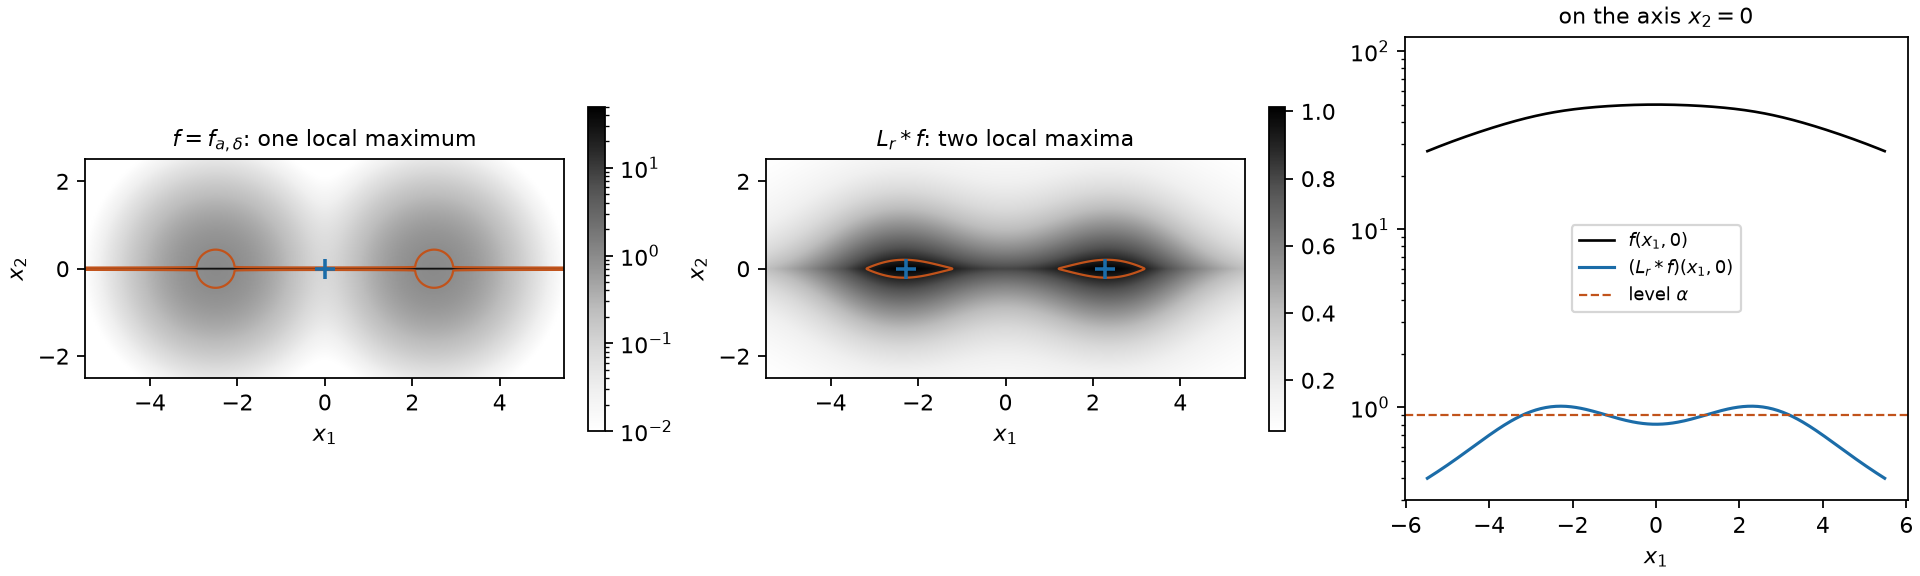
\includegraphics[width=\textwidth]{theory-creation.png}
\caption{Proposition~\ref{prop:creation-plane}(1) at $d = 2$ for the octave step $\mu = L_r$ of
the \Matern{} pyramid, $r = 1$, and the witness $f = f_{a,\delta}$ at $a = 5/2$, $\delta = 1/100$.
Left: $f$ on a logarithmic grey scale, with its one local maximum at $0$. Middle: $L_r * f$,
computed by the transform $(1 + r^2|\omega|^2)^{-1}$ on the periodic box
$[-18, 18] \times [-8, 8]$, sampled at the spacings $0.04$ along $x_1$ and $\delta/6$ along $x_2$
($900 \times 9600$ points), with two local maxima on that grid, at $(\pm2.28, 0)$. A grid point
counts as a local maximum when no neighbour of its $3 \times 3$ block is larger and its value
exceeds $10^{-3}$ of the maximum. These counts are computed. The proposition proves at least two
local maxima. The orange curves are the level $\alpha = 0.909$, midway between the value of
$L_r * f$ at $0$ and at its maxima. The set $\{f > \alpha\}$ is two discs joined by the thin strip
along the ridge, and $\{L_r * f > \alpha\}$ has two components. Right: both functions on the axis
$x_2 = 0$. By the proof of clause (3), $f$ is the record $\mu_s * g$ of the \Matern{} pyramid at
the scale $s$ with $cs = r$, so the middle panel is the next record $\mu_{qs} * g$. Let
$W := L_r * e^{-|\cdot|^2/2}$. The proof chooses a radius outside which $W < W(0)/4$, and it puts
$a$ one above that radius. Its argument needs only $a$ above the radius. Here $W = W(0)/4$ at
$2.331$, so $a = 5/2$ is admissible with any radius in $[2.331, 2.5)$. The proof's bound on the
ridge needs $\delta$ below about $0.002$, smaller than the $\delta$ drawn.}
\label{fig:theory-creation}
\end{figure}

A pyramid computed on a grid reads local maxima on the lattice, by comparing a value with the
values at finitely many neighbours. The next proposition carries the creation to that setting, in
$d \ge 2$. It covers one smoothing step by a mask. For an integer ratio $q \ge 2$ it also covers
the same step followed by decimation, and, for an infinitely divisible mask, every level of a
decimated pyramid.

% shared with blueprint prop:creation-grid
\begin{proposition}[creation on a grid]
\label{prop:creation-grid}

Let $d \ge 2$, let $w \ne \delta_0$ be a symmetric probability law on $h\ZZ^d$, and let
$\mathcal{N} \subset h\ZZ^d \setminus \{0\}$ be finite and symmetric and
contain the $2d$ axis neighbours. Call $x$ an \emph{$\mathcal{N}$-maximum} of $u$ if
$u(x) \ge u(x + y)$ for all $y \in \mathcal{N}$.
\begin{enumerate}
\item There is a summable $f > 0$ on $h\ZZ^d$ with exactly one $\mathcal{N}$-maximum such that
$w * f$ has at least two.
\item For an integer $q \ge 2$, $f$ can be chosen so that $(w * f)|_{qh\ZZ^d}$ has at least two
$q\mathcal{N}$-maxima as well.
\item If $w$ is infinitely divisible and $q \ge 2$ is an integer, then for every integer $k \ge 0$
every bounded array on $q^kh\ZZ^d$ is the level-$k$ record, smoothed and decimated $k$ times, of a bounded input on
$h\ZZ^d$: with $f_0$ the input, $f_j := \bigl((D_{q^{j-1}}w) * f_{j-1}\bigr)|_{q^jh\ZZ^d}$ and the
array $f_k$.
\end{enumerate}
\end{proposition}

\begin{proof}
Take $h = 1$, and write $|y|_1 := \sum_j|y_j|$.

\emph{An axis line of mass below one.} If every axis line $\ZZ e_j$ had mass $1$, $w$ would be
carried by their intersection $\{0\}$, as $d \ge 2$, and $w = \delta_0$. So some axis line
$\ZZ e_j$ has mass $p < 1$. The argument is written for $j = 1$; for another $j$ it is the same with
the coordinates $x_1$ and $x_j$ exchanged in the witness below, $\mathcal{N}$ entering only through
the $2d$ axis neighbours it contains. Put $\theta := 2/(1 + p)$, so that $\theta > 1$ and
$1 - \theta p = (1 - p)/(1 + p) > 0$.

\emph{The witness.} Write $x = (x_1, x')$ and $|x'|_1 := \sum_{j \ge 2}|x_j|$. Let
$\Psi(t) := \min(1 + |t|, 2e^{1 - |t|})$. It is $1 + |t|$ for $|t| \le 1$ and $2e^{1 - |t|}$
otherwise, it lies in $(0, 2]$, and $|\Psi(s) - \Psi(t)| \le 6|s - t|$. For an integer $R \ge 1$ put
\[
  b(x) := \Psi(x_1/R)\,e^{-|x'|_1/R}, \qquad
  f(x) := b(x) + \mathbf{1}_{\{x' = 0\}}\,\theta\max(1 - |x_1|/R, 0) .
\]
It is positive and even, and summable, as $f(x) \le (2 + \theta)e\,e^{-|x|_1/R}$.

\emph{One $\mathcal{N}$-maximum.} First $f(0) = 1 + \theta \ge f(x)$ for every $x$. Off the line
$f = b \le 2$. On it, $f(x) = 1 + \theta - (\theta - 1)|x_1|/R$ when $|x_1| \le R$, and $f \le 2$
beyond. So $0$ is an $\mathcal{N}$-maximum. From every $x \ne 0$ one axis step strictly raises $f$.
If $x' \ne 0$, a step toward the line in a coordinate $j \ge 2$ with $x_j \ne 0$ lowers $|x'|_1$ by
one, which raises $b$, and the ridge term cannot fall from $0$. If $x' = 0$ and $x_1 \ne 0$, the step
toward $0$ along the line raises $f$ by $(\theta - 1)/R$ while $|x_1| \le R$. Beyond, it raises $\Psi$
strictly, as $|x_1| - 1 \ge R$ (both are integers), and the ridge term is $0$ at $x$. As
$\mathcal{N}$ contains the axis neighbours, no $x \ne 0$ is an $\mathcal{N}$-maximum.

\emph{Two for the output.} The output $u := w * f$ is even, as $w$ is symmetric and $f$ even. It is
positive, and it tends to $0$ at infinity, by dominated convergence, as $f$ does. So $u$ attains its
maximum, and a maximizer is an $\mathcal{N}$-maximum for every $\mathcal{N}$. If $u(z) > u(0)$ for
some $z$, a maximizer $x^* \ne 0$ exists, and $-x^* \ne x^*$ is a second one. Now
$|b(x - y) - b(x)| \le \min(6|y|_1/R, 2)$, so
$\varepsilon(R) := \sum_yw(y)\min(6|y|_1/R, 2)$ bounds $|w * b - b|$ at every point, and
$\varepsilon(R) \to 0$ as $R \to \infty$ by dominated convergence: this is the tightness of $w$. The
ridge term of $u$ at $0$ is at most $\theta$ times the mass $p$ of the line. So
\[
  u(0) \le b(0) + \varepsilon(R) + \theta p = 1 + \varepsilon(R) + \theta p, \qquad
  u(Re_1) \ge b(Re_1) - \varepsilon(R) = 2 - \varepsilon(R),
\]
and $u(Re_1) - u(0) \ge 1 - \theta p - 2\varepsilon(R) > 0$ for large $R$. For (2), take $R = qK$
with $K$ large. Then $Re_1 = q(Ke_1)$ is on $q\ZZ^d$, and the same argument applies to the even
function $m \mapsto u(qm)$, which tends to $0$ at infinity.

\emph{(3)} Being symmetric and infinitely divisible, $w$ has \Levy{} data $(A, \nu)$ and the
generating triplet $(2A, \nu, 0)$, by Lemma~\ref{lem:symmetric-levy-khintchine}:
$\widehat w(\omega) = e^{-\langle\omega, A\omega\rangle - \int(1 - \cos\langle\omega, x\rangle)\,\nu(dx)}$.
Being carried by $\ZZ^d$, it has $A = 0$, and $\nu$ is finite and carried by
$\ZZ^d \setminus \{0\}$ (Lemma~\ref{lem:lattice-infinitely-divisible}). Put $a(n) := \nu(\{n\})$, a
summable symmetric kernel, and $M := \sum_na(n)$. Then
$\widehat w(\vartheta) = e^{-\sum_na(n)(1 - \cos\langle n, \vartheta\rangle)} = e^{-M}e^{\widehat a(\vartheta)}$,
the transform $\widehat a$ being real. Put $m := e^M\sum_{k \ge 0}(-1)^ka^{*k}/k!$. The series
converges absolutely in $\ell^1(\ZZ^d)$, with norm at most $e^{2M}$, so
$\widehat m = e^Me^{-\widehat a} = 1/\widehat w$ and $\widehat{w * m} = 1 = \widehat{\delta_0}$. A
summable kernel is determined by its Fourier coefficients, so $w * m = \delta_0$. At $k = 0$ the
array is its own input. Let $k \ge 1$, and suppose that every bounded array on $q^{k-1}\ZZ^d$ is the
level-$(k-1)$ record of a bounded input. Given a bounded array on $q^k\ZZ^d$, extend it by $0$ to a
bounded $u$ on $q^{k-1}\ZZ^d$, and put $v := (D_{q^{k-1}}m) * u$, a bounded array on
$q^{k-1}\ZZ^d$, as $D_{q^{k-1}}m$ is summable. By the induction hypothesis $v$ is the level-$(k-1)$
record $f_{k-1}$ of a bounded input $f_0$. Its smoothing $(D_{q^{k-1}}w) * v$ is
$(D_{q^{k-1}}(w * m)) * u = u$, by associativity, so
$f_k = \bigl((D_{q^{k-1}}w) * f_{k-1}\bigr)|_{q^k\ZZ^d} = u|_{q^k\ZZ^d}$ is the given array.
\end{proof}

Clause (3) carries clauses (1) and (2) to every level of a decimated grid pyramid whose mask is
infinitely divisible and whose ratio is an integer. The input that clause (1) gives for the mask at
level $k$ is bounded. So it is the level-$k$ record of a bounded input on $h\ZZ^d$, and the next
smoothing step raises the count. Section~\ref{sec:price-masks} reads the proposition on the masks of
the grid pyramids: the discrete Helmholtz mask, the frame mask and the binomial masks
(Proposition~\ref{prop:creation-grid-masks}).

\subsection{The selection}
\label{sec:matern-selection}

Counting fails in the plane, so a pyramid for images needs another principle to choose its family.
This subsection gives one, and finds the family it selects.

What remains of non-creation in the plane is non-enhancement: smoothing does not raise a local
maximum or lower a local minimum. Its classical form requires $\partial_tu \le 0$ at a spatial local
maximum of the record, which needs a derivative in scale
\prog{V-selection v0.1}{Thm.~4.2(3), p.~31}. A pyramid has no derivative in scale, only its octave
steps. Read at one finite step from $s$ to $t$, the principle requires $(u_t - u_s)/(t - s) \le 0$
at each weak local maximum of the later record $u_t$. This is the implicit Euler discretization of
the classical form. It needs no continuum of scales, so it can be required of an octave step. A
step of a family from scale $s$ to scale $t$ is its \emph{stage} $\mu_{s,t}$, and the octave step
from $t$ to $qt$ is the stage $\mu_{t,qt}$, an \emph{octave stage}.

The two forms select different families. On the line, the derivative form required at every scale
selects the Gaussian ray, the families whose exponent is $a\omega^2$,
\prog{V-selection v0.1}{Thm.~4.2(3) and Cor.~4.4, pp.~31, 33}. Among the symmetric
rotation-invariant laws, the finite-step form holds exactly for the Helmholtz resolvents
$(I - \tau\Delta)^{-1}$, $\tau \ge 0$, the identity among them. It rejects every Gaussian stage
$N(0, 2aI)$, $a > 0$ (Proposition~\ref{prop:stage-lemma}(3) and
Theorem~\ref{thm:selection-stratum-two}(4)).
\begin{itemize}
\item Definition~\ref{def:implicit-euler-principle} states the finite-step principle, on the
continuum and on a lattice.
\item The stage lemma, Proposition~\ref{prop:stage-lemma}, finds the laws that have it. Among the
symmetric rotation-invariant laws they are the Helmholtz resolvents $(I - \tau\Delta)^{-1}$,
$\tau \ge 0$.
\item The selection theorem, Theorem~\ref{thm:selection-stratum-two}, requires the principle at
every octave stage of an isotropic family covariant under $q$, in the canonical discrete gauge. It
finds the \Matern{} pyramid, up to the gauge $\chi \in \mathcal{G}_q$.
\item Proposition~\ref{prop:principle-other-readings} says what the principle gives in place of the
octave stages. Required of a kernel, for the families with transforms
$\exp\bigl(-[F(t|\omega|) - F(s|\omega|)]\bigr)$, it gives octave steps that are not resolvents.
Required of every stage, it holds for no symmetric family.
\end{itemize}

% shared with blueprint def:implicit-euler-principle
\begin{definition}[the implicit-Euler maximum principle]
\label{def:implicit-euler-principle}

A symmetric probability measure $\mu$ on $\RR^d$ has the \emph{implicit-Euler maximum principle}
if for every real $f \in \mathcal{S}(\RR^d)$ the output $u := \mu * f$ has $u(x) \le f(x)$ at every
weak local maximum $x$ of $u$, and $u(x) \ge f(x)$ at every weak local minimum. Here $x$ is a
\emph{weak local maximum} of $u$ if $u(x) \ge u(y)$ for every $y$ in a neighbourhood of $x$, and a
\emph{weak local minimum} if it is a weak local maximum of $-u$. A stage $\mu_{s,t}$ of a
family has the principle if the measure $\mu_{s,t}$ has it. On a lattice $h\ZZ^d$, with
$\mathcal{N} \subset h\ZZ^d \setminus \{0\}$ finite and symmetric, a symmetric probability $\kappa$
on $h\ZZ^d$ has the principle \emph{on $\mathcal{N}$} if for every bounded real $f$ on $h\ZZ^d$ the
output $u := \kappa * f$ has $u(x) \le f(x)$ at every $\mathcal{N}$-maximum $x$ of $u$ and
$u(x) \ge f(x)$ at every $\mathcal{N}$-minimum. Here $x$ is an \emph{$\mathcal{N}$-maximum} of $u$ if
$u(x) \ge u(x + y)$ for every $y \in \mathcal{N}$, and an \emph{$\mathcal{N}$-minimum} if it is an
$\mathcal{N}$-maximum of $-u$.
\end{definition}

The inputs are signed, so the clause at minima is the clause at maxima applied to $-f$.

The first task is to find the laws that have the principle. The answer is the stage lemma below.
On the continuum the principle holds for the resolvent of every positive semidefinite quadratic
form, and the converse shows that no symmetric probability measure on $\RR^d$ other than these
resolvents has it. On a lattice it holds for the resolvent of the $(2d+1)$-point Laplacian, read on
the $2d$ axis neighbours.

Why the principle selects the resolvents can be seen before the proof. The sufficiency is the
classical maximum principle of an elliptic equation. If
$\widehat\mu(\omega) = (1 + \omega\cdot C\omega)^{-1}$, then $u = \mu * f$ solves
$u - \nabla\cdot(C\nabla u) = f$. For a Schwartz input $u$ is smooth, since its derivatives are
$\mu * \partial^\alpha f$, whether or not $\mu$ has a bounded density. At a local maximum the
Hessian of $u$ is negative semidefinite, so $f - u = -\operatorname{tr}(C\nabla^2u) \ge 0$. The
converse tests the principle on inputs that are finite sums of cosines damped by a wide Gaussian,
chosen so that their limit outputs have a strict maximum at $0$. In the limit the principle becomes
a linear inequality on the values of $\widehat\mu$ at finitely many frequencies, with real weights of
either sign. A step of the proof shows that $\widehat\mu$ has no zero. Testing with suitable pairs of
frequencies then forces $1/\widehat\mu - 1$ to be a positive semidefinite quadratic form.

The sufficiency has a counterpart in regularization: Scherzer and Weickert read one regularization
step as one implicit diffusion step and prove its extremum principle
[\sscite{scherzer2000relations}, p.~43, and Lemma~6, p.~53]. The converse has two counterparts on
generators. An operator $A$ has the \emph{local positive maximum principle} if $Af(x) \le 0$
wherever $f$ has a local maximum $f(x) \ge 0$. A linear operator from smooth functions of compact
support to continuous functions with this principle is a second-order differential operator
[\sscite{courrege1966sur}, Thm.~0.1, p.~2-01]. Alvarez, Guichard, Lions and Morel derive a
second-order generator from a comparison principle and locality
[\sscite{alvarez1993axioms}, Thm.~2, p.~211]. The stage lemma reads its principle on one finite
step, a convolution, where these results read theirs on a generator.

% TODO(module C): cite prop:stage-lemma when released
The lemma belongs to the author's work on spatial scale space that is not yet published, so it is
stated here with its proof.

% shared with blueprint prop:stage-lemma
\begin{proposition}[the stage lemma]
\label{prop:stage-lemma}

Let $\mu$ be a symmetric probability measure on $\RR^d$.
\begin{enumerate}
\item \emph{(Sufficiency.)} For every positive semidefinite matrix $C$ there is a symmetric
probability measure with transform $(1 + \omega\cdot C\omega)^{-1}$, and it has the principle. In
particular the Helmholtz resolvent $(I - \tau\Delta)^{-1}$ has it for every $\tau \ge 0$, in every
dimension.
\item \emph{(The grid.)} On $h\ZZ^d$ the resolvent $\kappa$ of the $(2d+1)$-point Laplacian, with
transform $\bigl(1 + 4\tau h^{-2}\sum_{j=1}^d\sin^2(h\omega_j/2)\bigr)^{-1}$, $\tau \ge 0$, is a
symmetric probability and has the principle on the $2d$ axis neighbours.
\item \emph{(Converse.)} If $\mu$ has the principle, then $1/\widehat\mu(\omega) = 1 + \omega\cdot
C\omega$ for a positive semidefinite $C$. If $\mu$ is rotation invariant, $C = \tau I$ and $\mu$ is
the Helmholtz resolvent, the identity when $\tau = 0$.
\end{enumerate}
\end{proposition}

\begin{proof}
\emph{(1)} Write a positive semidefinite $C$ as $B^{\tp}B$, $B$ real, and put
$b_k := B^{\tp}e_k$, so that $\omega\cdot C\omega = |B\omega|^2 = \sum_k(\omega\cdot b_k)^2$. The
image $\mu_C$ of $L_1$ under $y \mapsto B^{\tp}y$ is a probability measure with the transform
$\widehat{L_1}(B\omega) = (1 + \omega\cdot C\omega)^{-1}$ (Lemma~\ref{lem:bessel-profile}(1)), which
is even, so $\mu_C$ is symmetric by the uniqueness of the transform.

Let $f \in \mathcal{S}(\RR^d)$ be real, and put $u := \mu_C * f$. The transform of $f$ is
$\widehat f(\omega) := \int e^{i\omega\cdot x}f(x)\,dx$, the transform of the measure $f(x)\,dx$, so
that Fourier inversion reads
$f(z) = (2\pi)^{-d}\int e^{-i\omega\cdot z}\widehat f(\omega)\,d\omega$. By Fubini's theorem $u$ has
the transform $\widehat{\mu_C}(\omega)\widehat f(\omega) =: g(\omega)$. As
$0 < \widehat{\mu_C} \le 1$ and $\widehat f$ is rapidly
decreasing, $g$ and $|\omega|^2g$ are integrable, and by Fourier inversion
\[
  u(z) = (2\pi)^{-d}\int e^{-i\omega\cdot z}g(\omega)\,d\omega, \qquad
  f(z) = (2\pi)^{-d}\int e^{-i\omega\cdot z}(1 + \omega\cdot C\omega)\,g(\omega)\,
  d\omega .
\]
These integrals are real, as $u$ and $f$ are; the real part written below only makes that
visible. So $f(x) - u(x) = (2\pi)^{-d}\sum_kQ_{b_k}$ with $Q_v := \operatorname{Re}\int e^{-i\omega\cdot x}
(\omega\cdot v)^2g(\omega)\,d\omega$. For a vector $v$ and $s \ne 0$,
\[
  \frac{u(x + sv) + u(x - sv) - 2u(x)}{s^2} = (2\pi)^{-d}\operatorname{Re}\int e^{-i\omega\cdot x}\,
  \frac{2\cos(s\,\omega\cdot v) - 2}{s^2}\,g(\omega)\,d\omega .
\]
The fraction in the integrand tends to $-(\omega\cdot v)^2$ as $s \to 0$ and is bounded by
$(\omega\cdot v)^2 \le |v|^2|\omega|^2$, as $1 - \cos y \le y^2/2$, so by dominated convergence the
quotient tends to $-(2\pi)^{-d}Q_v$. At a local maximum $x$ of $u$ its numerator is $\le 0$ for
small $s$, so $Q_v \ge 0$ for every $v$, and $f(x) \ge u(x)$. Minima follow with $-f$. The
Helmholtz resolvent is $C = \tau I$.

\emph{(2)} At $\tau = 0$, $\kappa = \delta_0$. Let $\tau > 0$, put $a := \tau h^{-2}$ and
$p := 2da/(1 + 2da) \in (0, 1)$, and let $\sigma$ be the simple random walk step, of mass $1/(2d)$ at
each $\pm he_j$, with transform $\widehat\sigma(\omega) = d^{-1}\sum_j\cos(h\omega_j)$. The
measure $(1 - p)\sum_{k \ge 0}p^k\sigma^{*k}$ is a symmetric probability on $h\ZZ^d$, a convex
combination of such, with the transform $(1 - p)/(1 - p\widehat\sigma)$. Its reciprocal is
$1 + \frac{p}{1 - p}(1 - \widehat\sigma) = 1 + 2da\cdot d^{-1}\sum_j(1 - \cos h\omega_j) =
1 + 4\tau h^{-2}\sum_j\sin^2(h\omega_j/2)$. So it is $\kappa$, by the uniqueness of Fourier
coefficients.
Let $\Delta_hu(n) := h^{-2}\sum_j\bigl(u(n + he_j) - 2u(n) + u(n - he_j)\bigr)$. The series gives
$\kappa * \sigma = (\kappa - (1 - p)\delta_0)/p$, and $\Delta_h\kappa = 2dh^{-2}(\kappa * \sigma -
\kappa)$, so $\kappa - \tau\Delta_h\kappa = \delta_0$, since $(1 - p)(1 + 2da) = 1$. For bounded real
$f$, $u := \kappa * f$ is bounded and $\Delta_hu = (\Delta_h\kappa) * f$, by shifting the summation
index, $\kappa$ being summable. So $u - \tau\Delta_hu = f$. At a maximum $x$ of $u$ over the axis
neighbours every term $u(x \pm he_j) - u(x)$ is nonpositive, so $\Delta_hu(x) \le 0$ and
$f(x) \ge u(x)$. Minima follow with $-f$.

\emph{(3)}
Write $\rho := \widehat\mu$. It is real, since $\mu$ is symmetric, continuous, and $\rho(0) = 1$.
The sine integrates to $0$ against $\mu$, so for $w, x \in \RR^d$
\[
  \int\cos\langle w, x - y\rangle\,\mu(dy) = \rho(w)\cos\langle w, x\rangle .
\]
The principle is tested on the inputs $\sum_ka_k\cos\langle w_k, x\rangle e^{-s|x|^2}$, whose
outputs tend as $s \to 0$ to $\sum_ka_k\rho(w_k)\cos\langle w_k, x\rangle$. Step~1 turns it into an
inequality between finitely many values of $\rho$, Step~2 shows that $\rho$ has no zero, and
Step~3 that $1/\rho - 1$ is a nonnegative quadratic form.

\emph{Step 1: the inequality.} Let $a_1, \dots, a_n \in \RR$ and $w_1, \dots, w_n \in \RR^d$, put
$b_k := a_k\rho(w_k)$, and suppose that $\sum_kb_k\langle w_k, x\rangle^2 \ge c|x|^2$ for every $x$,
with $c > 0$. Then $\sum_kb_k \le \sum_ka_k$. Step~2 applies this to pairs $(a_k, w_k)$ of a
weight and a frequency.

For $s \in (0, 1]$ the input $f_s(x) := \sum_ka_k\cos\langle w_k, x\rangle\,e^{-s|x|^2}$ is a real
Schwartz function, a Gaussian times functions whose derivatives are all bounded. Put
$h(x) := \sum_kb_k\cos\langle w_k, x\rangle$ and $A := \sum_k|a_k|$. By the identity above, and as
$|x - y| \le 1 + |y|$ for $|x| \le 1$,
\[
  \bigl|(\mu * f_s)(x) - h(x)\bigr| \le A\int\bigl(1 - e^{-s|x - y|^2}\bigr)\,\mu(dy)
  \le A\int\bigl(1 - e^{-s(1 + |y|)^2}\bigr)\,\mu(dy) \qquad (|x| \le 1),
\]
and the right side tends to $0$ as $s \to 0$, by dominated convergence. Next, $|\cos y - 1 +
y^2/2| \le y^4$ for $|y| \le 1$. With $K := \sum_k|b_k||w_k|^4$, as long as $|x||w_k| \le 1$ for
every $k$,
\[
  h(x) \le h(0) - \tfrac12\sum_kb_k\langle w_k, x\rangle^2 + K|x|^4
  \le h(0) - \tfrac c2|x|^2 + K|x|^4 ,
\]
so there is $r_0 \in (0, 1]$ with $h(x) \le h(0) - \frac c4|x|^2$ for $|x| \le r_0$. Let
$0 < r \le r_0$, and choose $s \in (0, 1]$ with $|\mu * f_s - h| < cr^2/8$ on the unit ball. The output
$u := \mu * f_s$ is continuous, so it attains its maximum over the closed ball of radius $r$ at some
point $x_s$. On the sphere $|x| = r$, $u(x) < h(x) + cr^2/8 \le h(0) - cr^2/8 < u(0)$, so
$|x_s| < r$, and $x_s$ is a local maximum of $u$. The principle gives
$h(0) - cr^2/8 < u(0) \le u(x_s) \le f_s(x_s)$. From $1 - y^2/2 \le \cos y \le 1$ and
$1 - e^{-t} \le t$, $f_s(x) \le \sum_ka_k + A_1|x|^2$ with $A_1 := \sum_k|a_k|(|w_k|^2/2 + 1)$.
Hence $\sum_kb_k = h(0) < \sum_ka_k + (A_1 + c/8)r^2$ for every $r \in (0, r_0]$, and
$\sum_kb_k \le \sum_ka_k$.

\emph{Step 2: $\rho$ has no zero.} By continuity there is $t > 0$ with $\rho(te_i) \ge \frac12$ for
$i = 1, \dots, d$. Suppose $\rho(\omega_0) = 0$, and apply Step~1 to the pairs $(1, te_i)$,
$i = 1, \dots, d$, and $(a_0, \omega_0)$. Whatever $a_0$, the hypothesis holds with $c = t^2/2$,
since $b_0 = a_0\rho(\omega_0) = 0$. The conclusion $\sum_i\rho(te_i) \le d + a_0$ fails for
$a_0 = -d - 1$.

\emph{Step 3: the reciprocal.} Put $m := 1/\rho - 1$. Step~1 with $a_k := b_k/\rho(w_k)$ reads: if
$\sum_kb_k\langle w_k, x\rangle^2 \ge c|x|^2$ for every $x$, with $c > 0$, then
$\sum_kb_km(w_k) \ge 0$. In the rest of this step a pair $(b_k, w_k)$ names the weight $b_k$ of this
form, not the weight $a_k$ of Step~1. If instead $\sum_kb_k\langle w_k, x\rangle^2 = 0$ for every $x$, the pairs
$(b_k, w_k)$ together with $(\varepsilon, e_i)$, $i = 1, \dots, d$, have the form $\varepsilon|x|^2$,
so $\sum_kb_km(w_k) + \varepsilon\sum_im(e_i) \ge 0$ for every $\varepsilon > 0$. The same holds
for $-b$, so $\sum_kb_km(w_k) = 0$. In the same way the pairs $(1, \omega)$ and
$(\varepsilon, e_i)$ give $m(\omega) \ge 0$. Let $C_{ij} := \frac12\bigl(m(e_i + e_j) - m(e_i) -
m(e_j)\bigr)$, a symmetric matrix. Fix $\omega$. The pair $(1, \omega)$ and, for all $i$ and $j$,
the pairs $(-\omega_i\omega_j/2, e_i + e_j)$, $(\omega_i\omega_j/2, e_i)$ and
$(\omega_i\omega_j/2, e_j)$ have the form $\langle\omega, x\rangle^2 -
\sum_{i,j}\omega_i\omega_jx_ix_j = 0$. So
$m(\omega) = \sum_{i,j}C_{ij}\omega_i\omega_j = \omega\cdot C\omega$. This is $\ge 0$ for every
$\omega$, so $C$ is positive semidefinite, and $1/\widehat\mu(\omega) = 1 + \omega\cdot C\omega$.

\emph{Rotation invariance.} If $\mu$ is rotation invariant, $\widehat\mu$ is radial, so
$\omega\cdot C\omega = \tau|\omega|^2$ with $\tau := e_1\cdot Ce_1 \ge 0$, and
$\widehat\mu(\omega) = (1 + \tau|\omega|^2)^{-1}$: $\mu$ is the Helmholtz resolvent. Any positive
semidefinite $C'$ with $1/\widehat\mu(\omega) = 1 + \omega\cdot C'\omega$ has the quadratic form
$\tau|\omega|^2$, so $C' = \tau I$, a symmetric matrix being determined by its quadratic form. When
$\tau = 0$, $\widehat\mu = 1$ and $\mu = \delta_0$, by the uniqueness of the transform.
\end{proof}

So a symmetric, rotation-invariant probability measure has the principle if and only if it is a
Helmholtz resolvent $(I - \tau\Delta)^{-1}$, $\tau \ge 0$. The converse assumes no infinite
divisibility and no other class of laws.

The lemma is about one law, and a pyramid has a whole ladder of octave stages. Between its knots a
family covariant under $q$ is in general not determined by its ladder, not even up to a relabelling
of the scales (Proposition~\ref{prop:ladder-knot-kernel}(2)). So the question is how much of a
family the principle fixes when it is required of its octave stages. The next theorem answers it
for an isotropic $q$-covariant family in the canonical discrete gauge. Required of one octave stage,
the principle fixes the ladder through it, and the stages between the rungs stay free. Required at
every octave stage $\mu_{t,qt}$, $t \in [1, q)$, it fixes the family up to the gauge
$\chi \in \mathcal{G}_q$, and full covariance follows. The last two clauses say which stages of the
\Matern{} pyramid have the principle. They also show that the Gaussian stages fail it, and so, in
$d \ge 2$, does the octave step of the frame \Matern{} pyramid.

% shared with blueprint thm:selection-stratum-two
\begin{theorem}[the selection, inside stratum 2]
\label{thm:selection-stratum-two}

Let $(\mu_{s,t})$ be an isotropic $q$-covariant family in dimension $d$, in the canonical discrete
gauge, with exponents $\Psi_t(|\omega|) := -\log\widehat{\mu_t}(\omega)$. Write $F^1_q$ for $F_q$ at
$c = 1$.
\begin{enumerate}
\item \emph{(One stage.)} For one $t > 0$, $\mu_{t,qt}$ has the principle if and only if
$\Psi_t(r) = \sum_{n \ge 1}\log(1 + \tau q^{-2n}r^2)$ for some $\tau > 0$. Then the whole ladder
through $t$ is that of the \Matern{} pyramid, $\mu_{q^kt,q^{k+1}t} = L_{\sqrt\tau q^k}$ for
$k \in \ZZ$, and the stages between the rungs are free: the isotropic $q$-covariant families in
the canonical discrete gauge with this ladder are not unique, and not unique up to a relabelling in
$\mathcal{G}_q$ either.
\item \emph{(Every octave stage.)} If $\mu_{t,qt}$ has the principle for all $t \in [1, q)$, then
there is $\chi \in \mathcal{G}_q$ with $\Psi_t = F^1_q(\chi(t)\,\cdot)$. So the family is the
\Matern{} pyramid of Theorem~\ref{thm:matern-pyramid} read in the gauge $\chi$, and it is fully
covariant, with $S_\lambda = \chi^{-1}(\lambda\chi)$. Conversely every such family has the
property.
\item \emph{(Which stages.)} Let $(\mu^{\mathrm M}_{s,t})$ be the \Matern{} pyramid of
Theorem~\ref{thm:matern-pyramid} with the constants $q$ and $c > 0$. Its stage
$\mu^{\mathrm M}_{s,t}$ with $0 < s < t$ has the principle if and only if $t = qs$, and
$\mu^{\mathrm M}_{0,t}$ with $t > 0$ never has it. In particular two octaves together fail, as does every stage
between other scales.
\item \emph{(Not selected.)} Let $c > 0$ and $t > 0$. A Gaussian stage $N(0, 2aI)$, $a > 0$, fails
the principle. The octave step at $t$ of the frame \Matern{} pyramid with the constant $c$
(Definition~\ref{def:frame-matern-pyramid}),
$\prod_j(1 + c^2t^2\omega_j^2)^{-1}$, fails it in $d \ge 2$, on the continuum, while each of its
axis passes has it.
\end{enumerate}
\end{theorem}

The proof of clause (2) recovers the gauge from the stages. At each starting scale $t$, clause (1)
gives the stage as $L_{\sqrt{\tau}}$ for a constant $\tau = \tau(t) > 0$, and
$\widehat{\mu_t}(\omega) = \exp(-F^1_q(\sqrt{\tau(t)}\,|\omega|))$. Covariance under $q$ gives
$\chi(qt) = q\chi(t)$ for $\chi := \sqrt\tau$. The cascade and (ND) make $\chi$ strictly increasing,
and continuity in scale makes it continuous. With $\chi(q^nt) = q^n\chi(t)$ it then maps
$(0, \infty)$ onto itself, so $\chi$ lies in $\mathcal{G}_q$.

\begin{proof}
\emph{(1)} The stage $\mu_{t,qt}$ is rotation invariant by (I3), and symmetric, $-I$ being
orthogonal, so Proposition~\ref{prop:stage-lemma}(3) gives
$\widehat{\mu_{t,qt}}(\omega) = (1 + \tau|\omega|^2)^{-1}$ with $\tau \ge 0$; and $\tau > 0$ by
(ND), as $\tau = 0$ makes $\mu_{t,qt} = \delta_0$. In the canonical discrete gauge
$D_q\mu_{0,t} = \mu_{0,qt}$, and $\mu_{0,qt} = \mu_{t,qt} * \mu_{0,t}$ by (I1), so
$\widehat{\mu_t}(q\omega) = (1 + \tau|\omega|^2)^{-1}\,\widehat{\mu_t}(\omega)$. Applied at
$q^{-n}\omega$, $n = 1, \dots, N$, this gives
\[
  \widehat{\mu_t}(\omega) = \widehat{\mu_t}(q^{-N}\omega)\prod_{n=1}^N
    \bigl(1 + \tau q^{-2n}|\omega|^2\bigr)^{-1} ,
\]
and $\widehat{\mu_t}(q^{-N}\omega) \to \widehat{\mu_t}(0) = 1$, as $\widehat{\mu_t}$ is
continuous. The product tends to $\exp\bigl(-\sum_{n \ge 1}\log(1 + \tau q^{-2n}|\omega|^2)\bigr)$,
the series converging since $\log(1 + x) \le x$. This is the form of $\Psi_t$, read on the
transform. Conversely, if $\Psi_t$ has that form, the series is $F^1_q(\sqrt\tau\,|\omega|)$, and
the telescoping $F^1_q(qr) = \log(1 + r^2) + F^1_q(r)$ gives
$\widehat{\mu_{t,qt}}(\omega) = \widehat{\mu_t}(q\omega)/\widehat{\mu_t}(\omega) =
(1 + \tau|\omega|^2)^{-1}$. So $\mu_{t,qt} = L_{\sqrt\tau}$ by Lemma~\ref{lem:bessel-profile}(1)
and the uniqueness of the transform, and it has the principle by
Proposition~\ref{prop:stage-lemma}(1). The stage at $q^kt$, $k \in \ZZ$, is the dilate
$D_{q^k}L_{\sqrt\tau} = L_{\sqrt\tau q^k}$, by covariance applied $|k|$ times.

For the freedom between the rungs it suffices to take $t = 1$. If $(\mu'_{s,u})$ is an isotropic
$q$-covariant family with $S_qu = qu$ and the steps $\mu'_{q^k,q^{k+1}} = L_{\sqrt\tau q^k}$,
$k \in \ZZ$, then $(\mu'_{s/t,u/t})$ is one with the ladder through $t$ of (1). A relabelling by
$g \in \mathcal{G}_q$ between two families so rescaled is a relabelling by
$u \mapsto g(tu)/t$, again in $\mathcal{G}_q$, between the families before rescaling. So it
suffices to build two isotropic families with $S_qu = qu$ and the ladder $(L_{\sqrt\tau q^k})_k$
that are not relabellings of each other by any element of $\mathcal{G}_q$.
Proposition~\ref{prop:ladder-knot-kernel}(2) gives them for the step $\varrho := L_{\sqrt\tau}$.

Let $\nu$ be the measure with the radial density
$b_d(|x|/\sqrt\tau)\bigl(|S^{d-1}|\,|x|^d\bigr)^{-1}$. By Lemma~\ref{lem:bessel-profile}(2) at
$\beta = \tau$, $\int(1 - \cos\langle\omega, x\rangle)\,\nu(dx) = \log(1 + \tau|\omega|^2)$.
In polar coordinates $\int(1 \wedge |x|^2)\,\nu(dx) = \int_0^\infty(1 \wedge r^2)\,b_d(r/\sqrt\tau)\,dr/r$,
which is finite since $b_d \le 2$ and $b_d(y) \le C_de^{-y/2}$ (Lemma~\ref{lem:bessel-profile}(3)).
So $\nu$ is a rotation-invariant \Levy{} measure, and the infinitely divisible law with the data
$(0, \nu)$ has the transform $(1 + \tau|\omega|^2)^{-1}$. It is $\varrho$, by
Lemma~\ref{lem:bessel-profile}(1), so $\varrho$ is symmetric, rotation invariant, infinitely
divisible and not $\delta_0$. Its logarithmic moment is finite, since $\log_+ r \le r$ and so
$\log_+ r\,b_d(r/\sqrt\tau)/r \le C_d e^{-r/(2\sqrt\tau)}$. Split $\nu = \nu_a + \nu_b$, with
$\nu_a$ the restriction of $\nu$ to $\{|x| \le 1\}$ and $\nu_b$ its restriction to $\{|x| > 1\}$.
Both are symmetric and rotation invariant, carried by disjoint sets, and nonzero since $b_d > 0$.
By Proposition~\ref{prop:ladder-knot-kernel}(2) there are two isotropic $q$-covariant families
with $S_qu = qu$ and the step $\mu_{1,q} = \varrho$, neither a relabelling of the other by an
element of $\mathcal{G}_q$. Covariance gives their ladder,
$\mu_{q^k,q^{k+1}} = D_{q^k}L_{\sqrt\tau} = L_{\sqrt\tau q^k}$. This is the last sentence of (1).

\emph{(2)} Every stage $\mu_{t,qt}$, $t > 0$, has the principle. With $q^nt \in [1, q)$, clause (1)
makes the stage at $q^nt$ the law $L_{\sqrt\tau}$, and the stage at $t$ is its dilate
$L_{\sqrt\tau q^{-n}}$, which has the principle by Proposition~\ref{prop:stage-lemma}(1). So clause
(1) applies at every $t > 0$: $\widehat{\mu_t}(\omega) = \exp(-F^1_q(\chi(t)|\omega|))$ with
$\chi(t) := \sqrt{\tau(t)} > 0$, since $\sum_n\log(1 + \tau q^{-2n}r^2) = F^1_q(\sqrt\tau r)$. As
$F^1_q$ is strictly increasing on $[0, \infty)$, $\chi(t)$ is read off $\widehat{\mu_t}(e)$ at a
unit vector $e$, and covariance, $D_{q^n}\mu_{0,t} = \mu_{0,q^nt}$, gives
$\chi(q^nt) = q^n\chi(t)$ for $n \in \ZZ$. If $\chi(t) \le \chi(s)$ with $s < t$, then by (I1)
$\widehat{\mu_{s,t}}(\omega) = \exp\bigl(F^1_q(\chi(s)|\omega|) - F^1_q(\chi(t)|\omega|)\bigr) \ge 1$.
A transform has modulus at most $1$, so $\widehat{\mu_{s,t}} = 1$ and $\mu_{s,t} = \delta_0$,
against (ND). So $\chi$ is strictly increasing on $(0, \infty)$. It is continuous there:
$\exp(-F^1_q(\chi(t))) = \widehat{\mu_t}(e)$ is continuous in $t$ by (I2), and if
$a' > \chi(t_0)$, then $F^1_q(a') > F^1_q(\chi(t_0))$, so $\chi(t) < a'$ for $t$ near $t_0$;
likewise from below. By the intermediate values $\chi([1, q]) \supseteq [\chi(1), q\chi(1)]$, and
with the dilations $\chi$ maps $(0, \infty)$ onto itself. So $\chi \in \mathcal{G}_q$, with
$\chi(0) := 0$. By (I1) the transforms are those of Theorem~\ref{thm:matern-pyramid} at $c = 1$ in
the gauge $\chi$,
$\widehat{\mu_{s,t}}(\omega) = \exp\bigl(-[F^1_q(\chi(t)|\omega|) - F^1_q(\chi(s)|\omega|)]\bigr)$,
and the transform determines the law. The map $S_\lambda := \chi^{-1}(\lambda\chi)$, with
$S_\lambda(0) := 0$, is an increasing bijection of $[0, \infty)$, and reading the transforms at
$\lambda\omega$ gives $D_\lambda\mu_{s,t} = \mu_{S_\lambda s, S_\lambda t}$ for every
$\lambda > 0$. Conversely, for such a family telescoping gives
$\widehat{\mu_{t,qt}}(\omega) = (1 + \chi(t)^2|\omega|^2)^{-1}$, so $\mu_{t,qt} = L_{\chi(t)}$ by
Lemma~\ref{lem:bessel-profile}(1) and the uniqueness of the transform, and
Proposition~\ref{prop:stage-lemma}(1) applies.

\emph{(3)} The stage $\mu^{\mathrm M}_{s,t}$, $0 \le s < t$, has the transform
$\exp\bigl(-[F_q(t|\omega|) - F_q(s|\omega|)]\bigr)$, real and even, so it is symmetric. If it
has the principle, Proposition~\ref{prop:stage-lemma}(3) along a unit vector $e$ gives
$\exp D(x) = 1 + kx^2$ for $x \ge 0$, with $D(x) := F_q(tx) - F_q(sx)$ and
$k := e\cdot Ce \ge 0$. The telescoping $F_q(qy) = \log(1 + c^2y^2) + F_q(y)$ at $y = tx$ and
$y = sx$ gives $D(qx) = D(x) + \log(1 + c^2t^2x^2) - \log(1 + c^2s^2x^2)$, so with $u = x^2$
\[
  (1 + kq^2u)(1 + c^2s^2u) = (1 + c^2t^2u)(1 + ku) , \qquad u \ge 0 .
\]
Both sides are polynomials in $u$ of degree at most $2$ with the constant term $1$, so their equality at $u = 1$ and $u = 2$ makes the coefficients of $u^2$ and of $u$ agree:
$kc^2(t^2 - q^2s^2) = 0$ and $c^2(t^2 - s^2) = k(q^2 - 1)$. If $k = 0$, the second gives $t = s$,
which is excluded; so $k > 0$, and the first gives $t = qs$. At $s = 0$ this reads $t = 0$, which is
excluded: $\mu^{\mathrm M}_{0,t}$ never has the principle. Conversely
$\mu^{\mathrm M}_{s,qs} = L_{cs}$ (Theorem~\ref{thm:matern-pyramid}(1)) has the principle by
Proposition~\ref{prop:stage-lemma}(1).

\emph{(4)} The Gaussian stage and the frame step have real even transforms, so they are symmetric.
If the Gaussian stage had the principle, Proposition~\ref{prop:stage-lemma}(3) along a unit vector
would give $e^{ax^2} = 1 + kx^2$ for every $x$; at $x = 1$ and $x = \sqrt2$,
$(1 + k)^2 = e^{2a} = 1 + 2k$, so $k = 0$ and $a = 0$, which is excluded. If the frame step had it,
the same proposition would give $\prod_j(1 + c^2t^2\omega_j^2) = 1 + \omega\cdot C\omega$. On the
diagonal $\omega = x(e_1 + e_2)$, which $d \ge 2$ allows, this reads
$(1 + Kx^2)^2 = 1 + Qx^2$ with $K := c^2t^2 > 0$ and $Q := (e_1 + e_2)\cdot C(e_1 + e_2)$; at
$x = 1$ and $x = \sqrt2$ it gives $2K^2 = 0$, which is excluded. The axis pass along $e_j$, the
Laplace law on the line $\RR e_j$ with transform $(1 + c^2t^2\omega_j^2)^{-1}$, is
Proposition~\ref{prop:stage-lemma}(1) with the degenerate $C = c^2t^2e_je_j^{\tp}$.
\end{proof}

Clause (4) is stated on the continuum. Its grid case is in Section~\ref{sec:price-obstruction}. On
$h\ZZ^d$, $d \ge 2$, the frame mask, which is the octave step of the frame \Matern{} pyramid on the
grid, fails the principle on every finite symmetric neighbourhood. Each of its axis passes has it on
every such neighbourhood that contains the two neighbours along its axis
(Proposition~\ref{prop:grid-frame-step-not-selected}).

A heuristic picture shows why a Gaussian stage fails. The proof of clause (4) does not use it. Take
a nonnegative input with two narrow bumps at $\pm be_1$ and nothing between them. A kernel with a
$C^2$ density and a nondegenerate maximum at $0$ merges them into one maximum at the origin, when
$b$ is small against its width and the bumps are narrow against $b$. There the output is positive
and the input is zero, so $u > f$ at a maximum. The Gaussian is such a kernel. The resolvent's
kernel is not smooth at its centre. It has a corner on the line and a singularity in the plane
(Proposition~\ref{prop:matern-generator-octave}(3)), so the picture does not apply to it. That the
resolvent passes is clause (1) of Proposition~\ref{prop:stage-lemma}.

In the plane, then, the case for the \Matern{} pyramid rests on non-enhancement read at a finite
step, through the converse of the stage lemma. Counting fails on the \Matern{} and frame \Matern{}
ladders, and at every rung of the Gaussian ladder (Section~\ref{sec:matern-counting}). It survives on
the projections of Theorem~\ref{thm:matern-pyramid}(3), for inputs whose projection has a version
that is the primitive of an integrable function. On a grid the resolvent of the $(2d+1)$-point
Laplacian has the principle on the $2d$ axis neighbours (Proposition~\ref{prop:stage-lemma}(2)).
The frame mask lacks it on every finite symmetric neighbourhood
(Proposition~\ref{prop:grid-frame-step-not-selected}).

The selection theorem requires the principle of the octave stages, and this is a choice. Two other
readings suggest themselves. The first requires it of the kernels $\mu_{0,t}$, read from the
origin. The second requires it of every stage. The next proposition shows that neither gives a
pyramid whose octave steps are resolvents. Its first clause covers the families with transforms
$\exp\bigl(-[F(t|\omega|) - F(s|\omega|)]\bigr)$, and its second every symmetric family.

% shared with blueprint prop:principle-other-readings
\begin{proposition}[the principle read from the origin and at every stage]
\label{prop:principle-other-readings}

Let $d \ge 1$.
\begin{enumerate}
\item \emph{(From the origin.)} Let $F$ be a real function on $[0, \infty)$ with $F(0) = 0$, not
identically $0$, and let
$(\mu_{s,t})$ be a family in dimension $d$ with
$\widehat{\mu_{s,t}}(\omega) = \exp\bigl(-[F(t|\omega|) - F(s|\omega|)]\bigr)$. If the kernel
$\mu_{0,t}$ has the principle for one $t > 0$, then $F(r) = \log(1 + \tau r^2)$ for some
$\tau > 0$, the \Matern{} family of index $1$, and then every kernel $\mu_{0,t}$ has it. Its octave
steps, with transform $(1 + \tau t^2|\omega|^2)/(1 + \tau q^2t^2|\omega|^2)$ for a ratio $q > 1$, are
not resolvents $(1 + \omega\cdot C\omega)^{-1}$.
\item \emph{(Every stage.)} No symmetric family in dimension $d$ has the principle at every stage
$\mu_{s,t}$, $0 \le s < t$.
\end{enumerate}
\end{proposition}

\begin{proof}
\emph{(1)} The kernel $\mu_{0,t}$ has the transform $e^{-F(t|\omega|)}$, as $F(0) = 0$, which is
real and even, so $\mu_{0,t}$ is symmetric. By Proposition~\ref{prop:stage-lemma}(3),
$1/\widehat{\mu_{0,t}}(\omega) = 1 + \omega\cdot C\omega$ with $C$ positive semidefinite. Along a
unit vector $e$, with $k := e\cdot Ce \ge 0$, this reads $e^{F(tx)} = 1 + kx^2$ for $x \ge 0$, so
$F(r) = \log(1 + \tau r^2)$ for $r \ge 0$, with $\tau := k/t^2 \ge 0$, and $\tau > 0$ as $F$ is not
identically $0$. Then $\widehat{\mu_{0,t'}}(\omega) = (1 + \tau t'^2|\omega|^2)^{-1}$ for every
$t' > 0$, which has the principle by Proposition~\ref{prop:stage-lemma}(1). Suppose the octave
step $\mu_{t',qt'}$, with transform $(1 + \tau t'^2|\omega|^2)/(1 + \tau q^2t'^2|\omega|^2)$, were
$(1 + \omega\cdot C'\omega)^{-1}$ for a real matrix $C'$. Along $e$, with $a := \tau t'^2 > 0$ and
$K := e\cdot C'e$, $(1 + ax^2)(1 + Kx^2) = 1 + aq^2x^2$ for $x \ge 0$. At $x = 1$ and $x = \sqrt2$
this gives $a + K + aK = aq^2$ and $2a + 2K + 4aK = 2aq^2$, so $aK = 0$, hence $K = 0$, and then
$a = aq^2$, $q = 1$, a contradiction.

\emph{(2)} Suppose every stage has the principle. By Proposition~\ref{prop:stage-lemma}(3) there
are positive semidefinite $C_1$, $C_2$, $C_3$ with
$1/\widehat{\mu_{0,1}} = 1 + \omega\cdot C_1\omega$, $1/\widehat{\mu_{1,2}} = 1 + \omega\cdot
C_2\omega$ and $1/\widehat{\mu_{0,2}} = 1 + \omega\cdot C_3\omega$. Write
$Q_i(\omega) := \omega\cdot C_i\omega \ge 0$. The cascade $\mu_{0,2} = \mu_{1,2} * \mu_{0,1}$,
read at $x\omega$, gives $(1 + x^2Q_1(\omega))(1 + x^2Q_2(\omega)) = 1 + x^2Q_3(\omega)$, and at
$x = 1$ and $x = \sqrt2$, as in (1), $Q_1(\omega)Q_2(\omega) = 0$ for every $\omega$. Write
$C_i = B_i^\top B_i$, so that $Q_i(\omega) = |B_i\omega|^2$ and a zero of $Q_i$ is in the kernel of
$B_i$. If $Q_1(\omega_1) > 0$ and $Q_2(\omega_2) > 0$, then $Q_2(\omega_1) = 0 = Q_1(\omega_2)$, so
$Q_1(\omega_1 + \omega_2) = Q_1(\omega_1) > 0$ and $Q_2(\omega_1 + \omega_2) = Q_2(\omega_2) > 0$,
against the product's vanishing at $\omega_1 + \omega_2$. So $Q_1 \equiv 0$ or $Q_2 \equiv 0$: then
$\widehat{\mu_{0,1}} \equiv 1$ or $\widehat{\mu_{1,2}} \equiv 1$, that is $\mu_{0,1} = \delta_0$ or
$\mu_{1,2} = \delta_0$, against (ND).
\end{proof}

Read from the origin, among the families with transforms
$\exp\bigl(-[F(t|\omega|) - F(s|\omega|)]\bigr)$, the principle selects one whose octave steps are
not resolvents. Read at every stage, it is satisfied by no symmetric family. Of the three readings, the ladder is the one under which
the octave steps are Helmholtz resolvents, and Theorem~\ref{thm:selection-stratum-two} takes it.

The principle bounds the value of the output at a weak local maximum by the input there. It says
nothing about the number of local maxima. The resolvent $L_{ct}$ has the principle and still
creates local maxima (Proposition~\ref{prop:creation-plane}(1)). On a grid the principle is proved
here for one smoothing step (Proposition~\ref{prop:stage-lemma}(2)). A pyramid decimates after
each step, and a local maximum of a decimated record need not be a local maximum on the finer grid.
For the $(2d+1)$-point resolvent and one finitely supported input, the inequality of the principle
fails at a maximum of the decimated output over its axis neighbours on the coarse grid.

% shared with blueprint prop:principle-after-decimation
\begin{proposition}[the pointwise principle after decimation]
\label{prop:principle-after-decimation}

Let $d \ge 1$, $h > 0$ and $\tau > 0$, let $\kappa$ be the resolvent of
Proposition~\ref{prop:stage-lemma}(2) on $h\ZZ^d$, and let $\Delta_h$ be the $(2d+1)$-point
Laplacian, $\Delta_hu(x) := h^{-2}\sum_{j=1}^d\bigl(u(x + he_j) - 2u(x) + u(x - he_j)\bigr)$. Let
$u(0) := 1$, $u(\pm he_j) := 2$ for $j = 1, \dots, d$, and $u := 0$ elsewhere on $h\ZZ^d$, and put
$f := u - \tau\Delta_hu$.
\begin{enumerate}
\item $\kappa * f = u$, and $f(0) = 1 - 2d\tau/h^2 < u(0)$.
\item \emph{(After decimation.)} For every integer $q \ge 2$, $u$ vanishes at the $2d$ axis
neighbours $\pm qhe_j$ of the origin in the coarse grid $qh\ZZ^d$, so the origin is a strict
maximum of $u$ restricted to $qh\ZZ^d$ over those neighbours, while $u(0) > f(0)$. The decimated
output and the decimated input, $u$ and $f$ restricted to $qh\ZZ^d$, fail the inequality
$u(x) \le f(x)$ of Definition~\ref{def:implicit-euler-principle} at that maximum.
\item \emph{(Before decimation.)} On $h\ZZ^d$ the origin is not a maximum of $u$ over its axis
neighbours, and the pair $(u, f)$ satisfies the principle on the $2d$ axis neighbours at every
point of $h\ZZ^d$, by Proposition~\ref{prop:stage-lemma}(2).
\end{enumerate}
\end{proposition}

\begin{proof}
\emph{(1)} First, $\kappa - \tau\Delta_h\kappa = \delta_0$. Both sides are summable on $h\ZZ^d$,
the transform of the left side is
$\bigl(1 + 4\tau h^{-2}\sum_{j=1}^d\sin^2(h\omega_j/2)\bigr)\widehat\kappa(\omega) = 1$, and a
summable function on $h\ZZ^d$ is determined by its transform. The function $u$ has finite support, so $u$ and
$\Delta_hu$ are summable, and $\Delta_h$ passes onto either factor of a convolution of summable
functions by shifting the summation index. So
\[
\kappa * f = \kappa * u - \tau\,\kappa * \Delta_hu = \kappa * u - \tau\,(\Delta_h\kappa) * u
= (\kappa - \tau\Delta_h\kappa) * u = u .
\]
At the origin, $\Delta_hu(0) = h^{-2}\sum_{j=1}^d(2 - 2 + 2) = 2dh^{-2}$, so
$f(0) = 1 - 2d\tau/h^2$, which is less than $u(0) = 1$ as $\tau > 0$.

\emph{(2)} The $j$-th coordinate of $\pm qhe_j$ is $\pm qh$, and $q \ge 2$, so $\pm qhe_j$ is neither
the origin nor one of the points $\pm he_k$. Hence $u(\pm qhe_j) = 0 < 1 = u(0)$, while
$u(0) > f(0)$ by (1).

\emph{(3)} $u(he_1) = 2 > 1 = u(0)$. The input $f$ has finite support, so it is bounded, and
$u = \kappa * f$ by (1). Proposition~\ref{prop:stage-lemma}(2) gives $u(x) \le f(x)$ at every
maximum of $u$ over the axis neighbours and $u(x) \ge f(x)$ at every minimum.

Every step is machine-checked, with no cited fact.
\end{proof}

